\chapter{First-order reversal curve diagram modelling of framboidal greigite}
\label{ch:res-4}

\section*{Abstract}
In this chapter...\par

\section{Introduction}
Introduction goes here...\par

\section{Methodology}
Outline of the methodology of this chapter...\par

\subsection{The micromagnetic method}
Outline of the micromagnetic method...Perhaps not needed and can reference other chapters since this is not really a paper yet?\par

\subsection{The FORC model}
Outline of the FORC model. Explain why the choice of 85 field directions on a sector of the sphere based on symmetry arguments. Explain how the fields are obtained with an unstructured mesh over the sector of the sphere. Explain the method of only calculating the FORCs starting on switching fields since all the particles are always SD and mostly rotate reversibly.\par
\begin{figure}
\centering
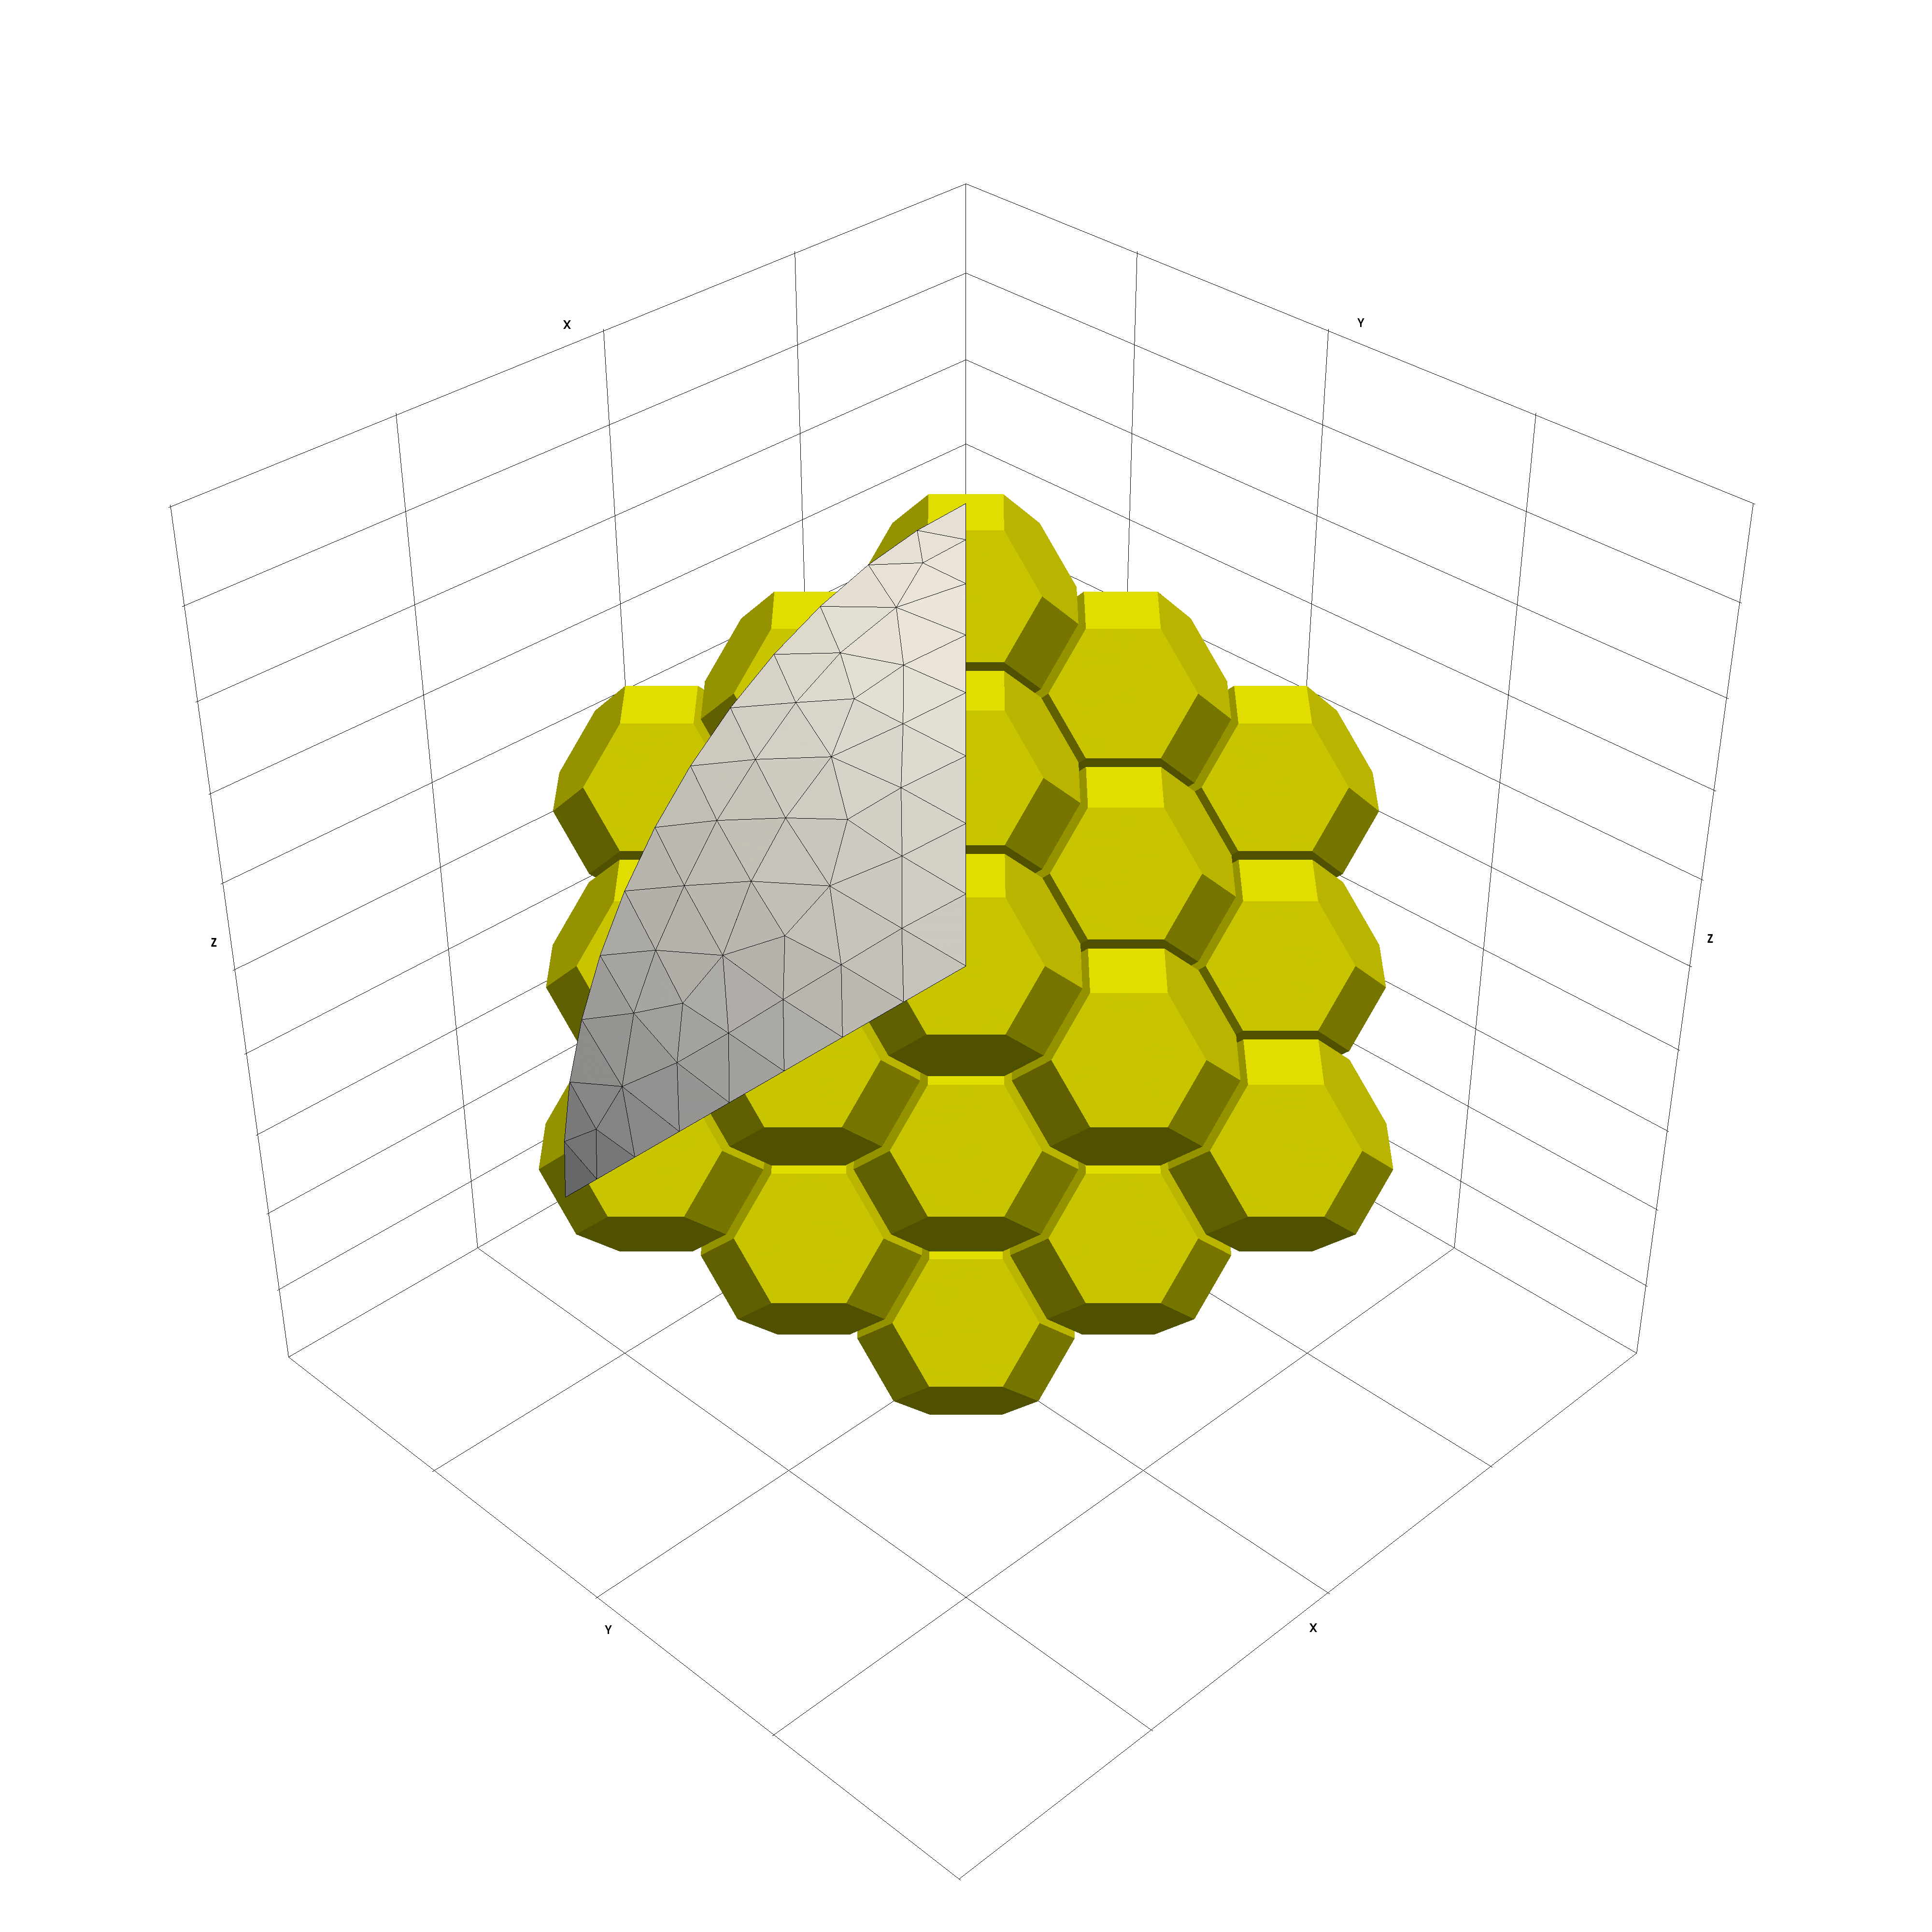
\includegraphics[width=\textwidth]{research-4/figs/mesh_orientations_HD.png}
\caption[Framboidal mesh and field orientations]{Framboidal mesh and field orientations.}
\label{FIG_01}
\end{figure}

\subsection{Mesh generation}
Outline of mesh generation. Explain the algorithm to produce arbitrarily large ordered framboidal meshes.\par

\section{Results}
Results section...\par

\subsection{The FORC diagrams}
Results of the hysteresis, FORCs and FORC diagrams. Explain here how the hysteresis curves (Figs. \ref{FIG_02}, \ref{FIG_04}, \ref{FIG_06}, \ref{FIG_08}) and FORC diagrams (Figs. \ref{FIG_03}, \ref{FIG_05}, \ref{FIG_07}, \ref{FIG_09}) depend on the field orientation. How the easy, hard axis are preserved in the framboidal structure (as compared to the isolated particles). Explain what the different FORC diagram features mean as switching fields of the individual particles in the framboids. Explain the FORCs (Fig. \ref{FIG_09}) and FORC diagram (Fig. \ref{FIG_10}) of the dispersion (ensemble average). Explain how FORC diagrams for mixtures of framboids and isolated SD particles (Fig. \ref{FIG_11}) and framboids and isolated SV particles (Fig. \ref{FIG_12}) were obtained (simple averages where the framboidal mass and isolated mass are the same). Explain how the framboids and the mixtures plot on the Day plot (Fig. \ref{FIG_14}).\par
\begin{figure}
\centering
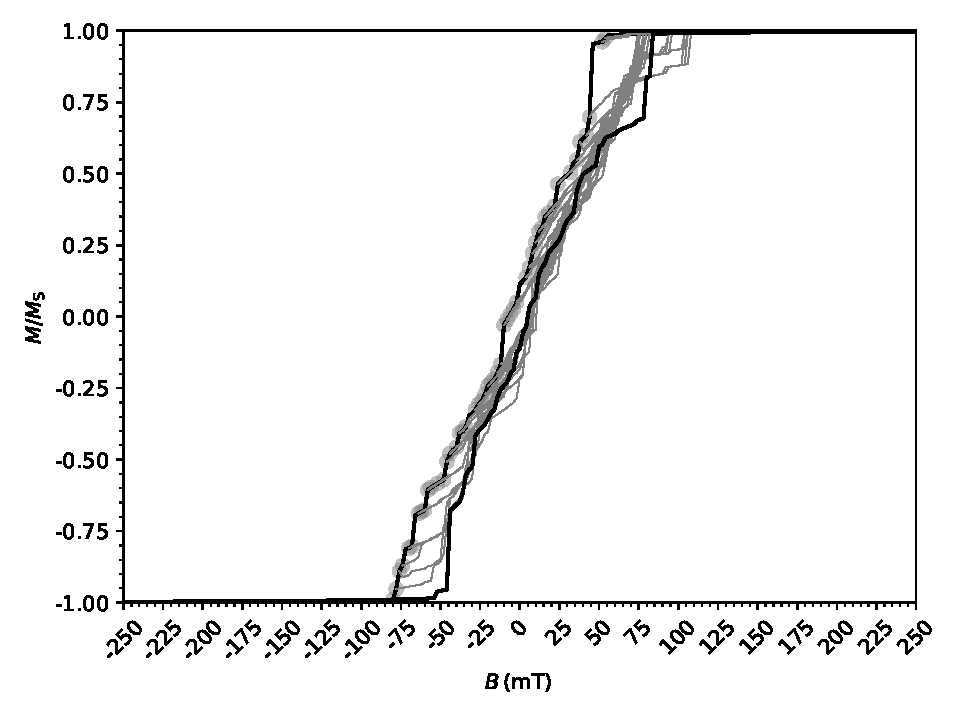
\includegraphics[width=\textwidth]{research-4/figs/BM21_withFORCS.pdf}
\caption[FORCs when the field is along an easy axis]{FORCs when the field is along an easy axis}.
\label{FIG_02}
\end{figure}

\begin{figure}
\centering
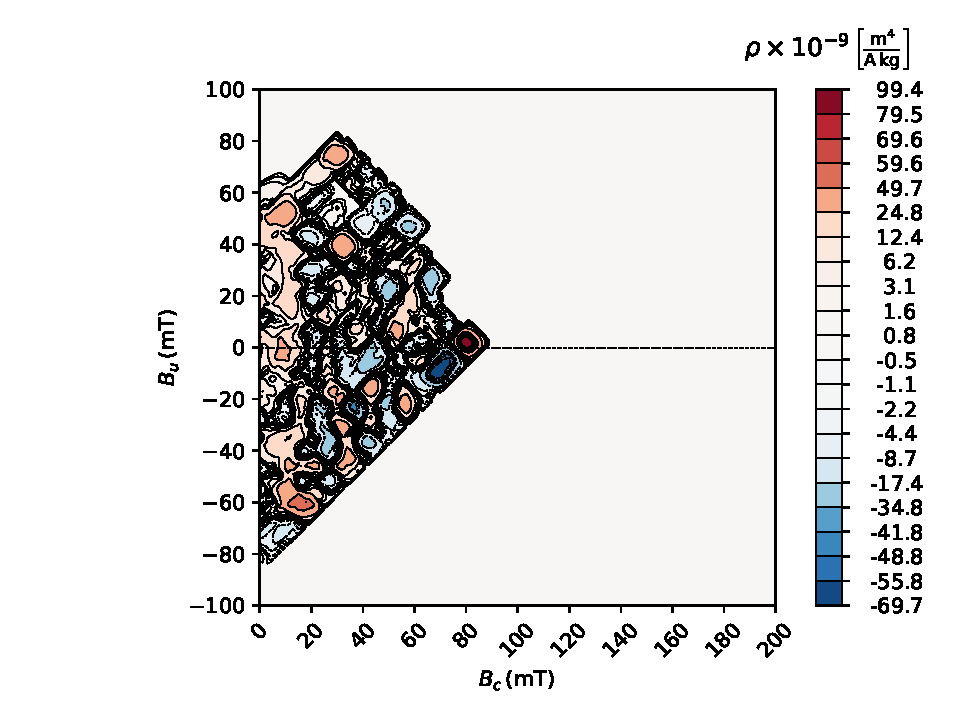
\includegraphics[width=\textwidth]{research-4/figs/FORC_21_SF4.pdf}
\caption[FORC diagram when the field is along an easy axis]{FORC diagram (SF=4) when the field is along an easy axis.}
\label{FIG_03}
\end{figure}

\begin{figure}
\centering
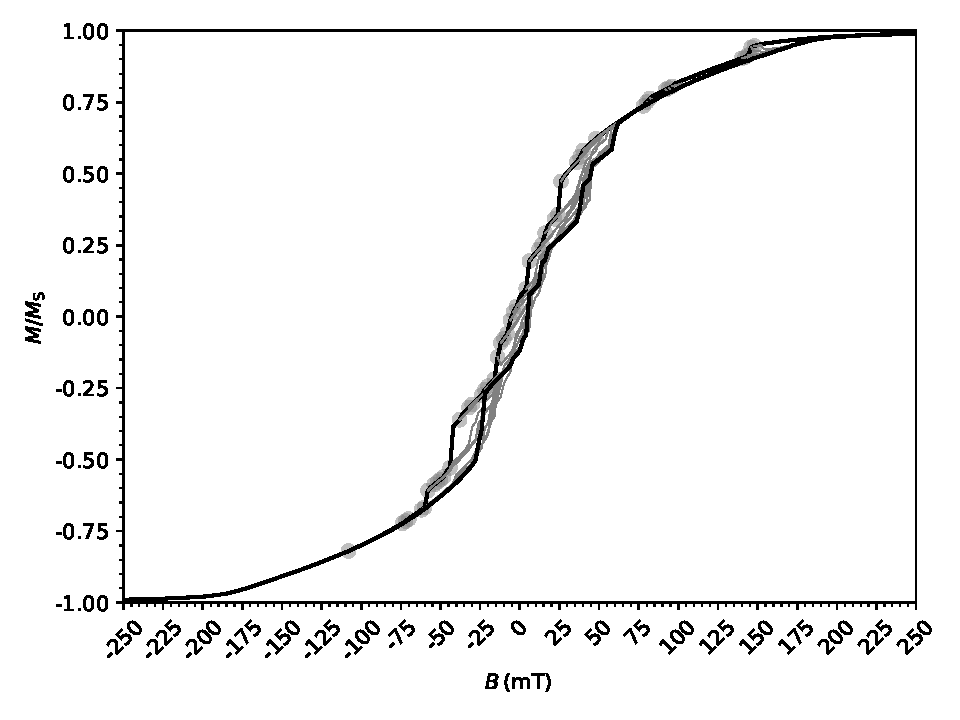
\includegraphics[width=\textwidth]{research-4/figs/BM16_withFORCS.pdf}
\caption[FORCs when the field is along a hard axis]{FORCs when the field is along a hard axis.}
\label{FIG_04}
\end{figure}

\begin{figure}
\centering
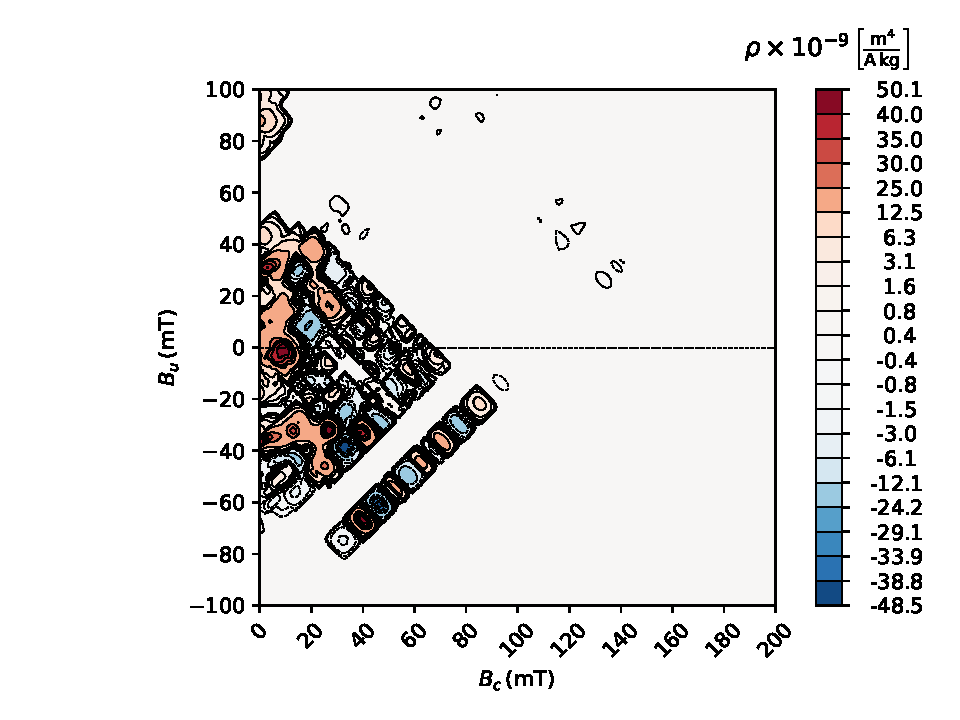
\includegraphics[width=\textwidth]{research-4/figs/FORC_16_SF4.pdf}
\caption[FORC diagram when the field is along a hard axis]{FORC diagram (SF=4) when the field is along a hard axis.}
\label{FIG_05}
\end{figure}

\begin{figure}
\centering
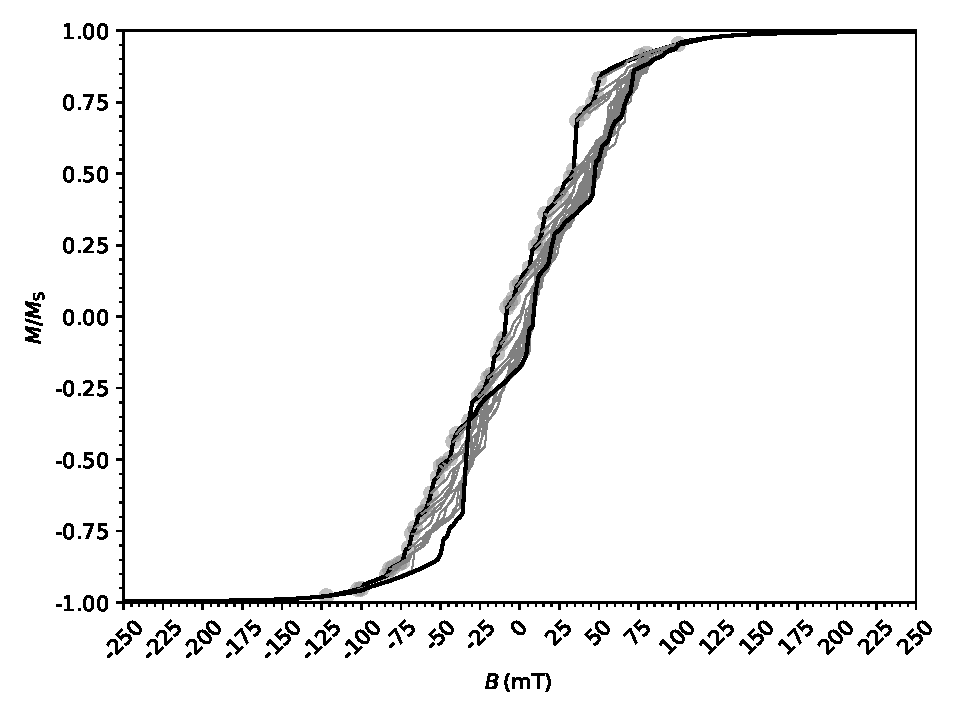
\includegraphics[width=\textwidth]{research-4/figs/BM14_withFORCS.pdf}
\caption[FORCs when the field is along a saddle point]{FORCs when the field is along a saddle point.}
\label{FIG_06}
\end{figure}

\begin{figure}
\centering
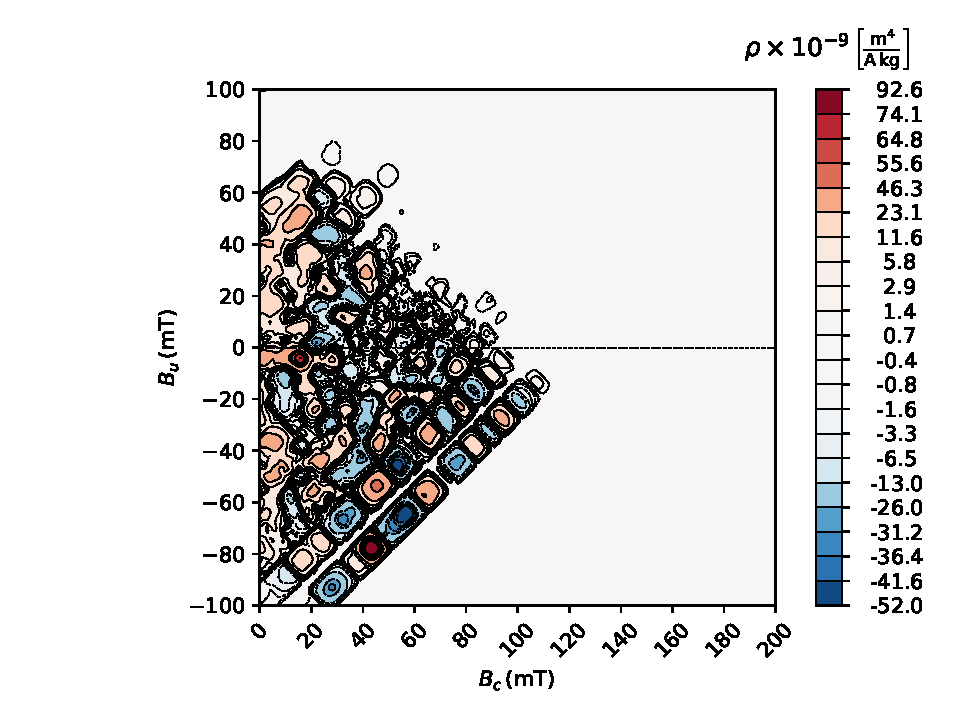
\includegraphics[width=\textwidth]{research-4/figs/FORC_14_SF4.pdf}
\caption[FORC diagram when the field is along a saddle point]{FORC diagram (SF=4) when the field is along a saddle point.}
\label{FIG_07}
\end{figure}

\begin{figure}
\centering
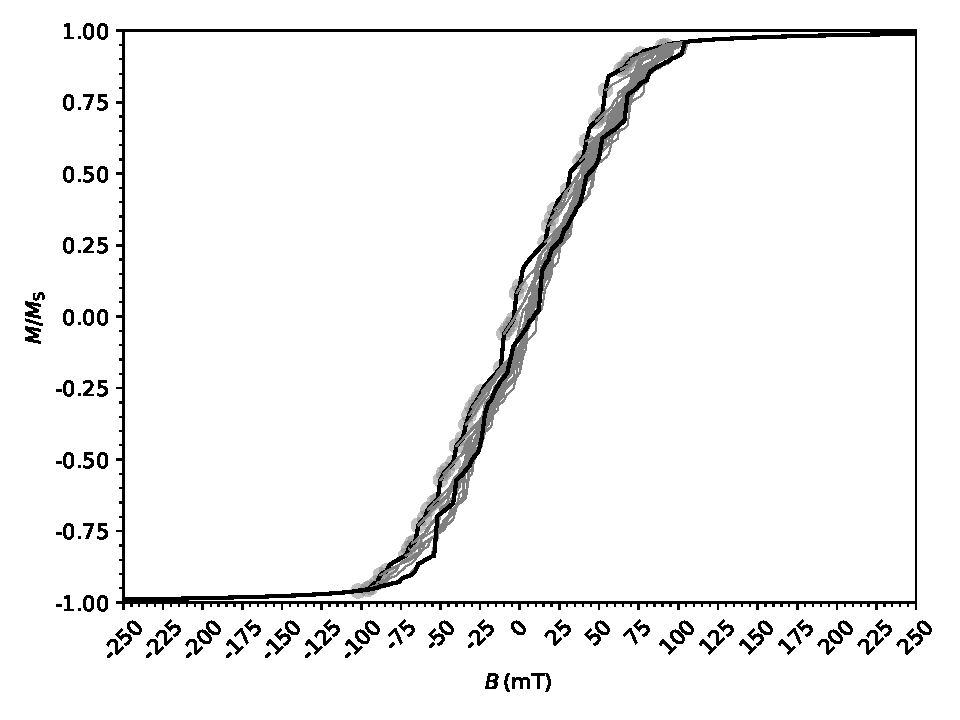
\includegraphics[width=\textwidth]{research-4/figs/BM53_withFORCS.pdf}
\caption[FORCs when the field is along a direction between easy, hard and saddle directions]{FORCs when the field is along a direction between easy, hard and saddle directions.}
\label{FIG_08}
\end{figure}

\begin{figure}
\centering
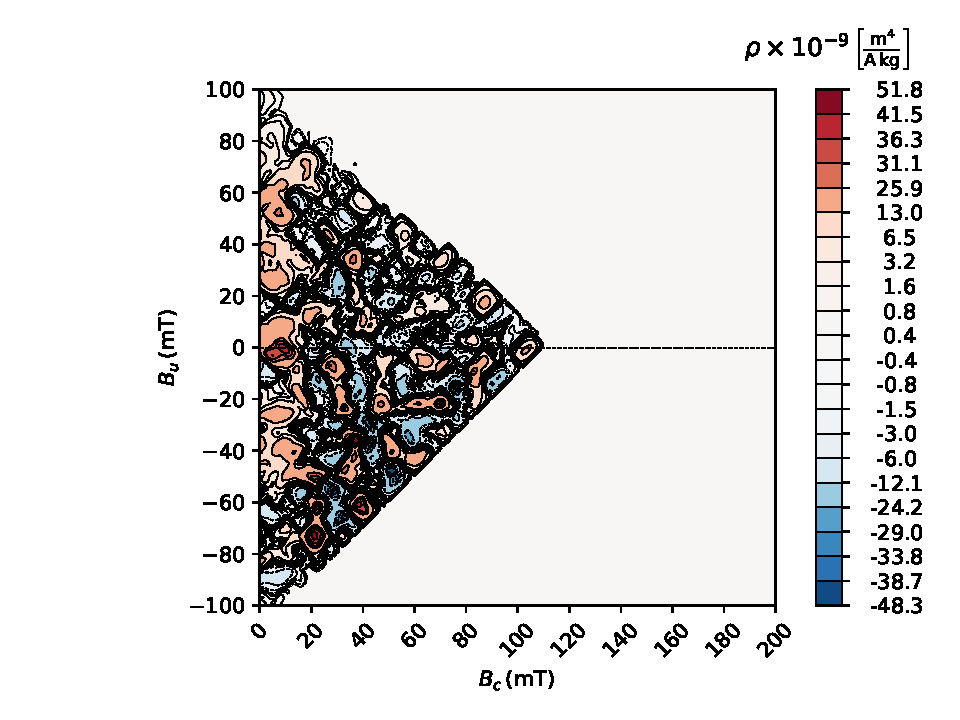
\includegraphics[width=\textwidth]{research-4/figs/FORC_53_SF4.pdf}
\caption[FORC diagram when the field is along a direction between easy, hard and saddle directions]{FORC diagram (SF=4) when the field is along a direction between easy, hard and saddle directions.}
\label{FIG_09}
\end{figure}

\begin{figure}
\centering
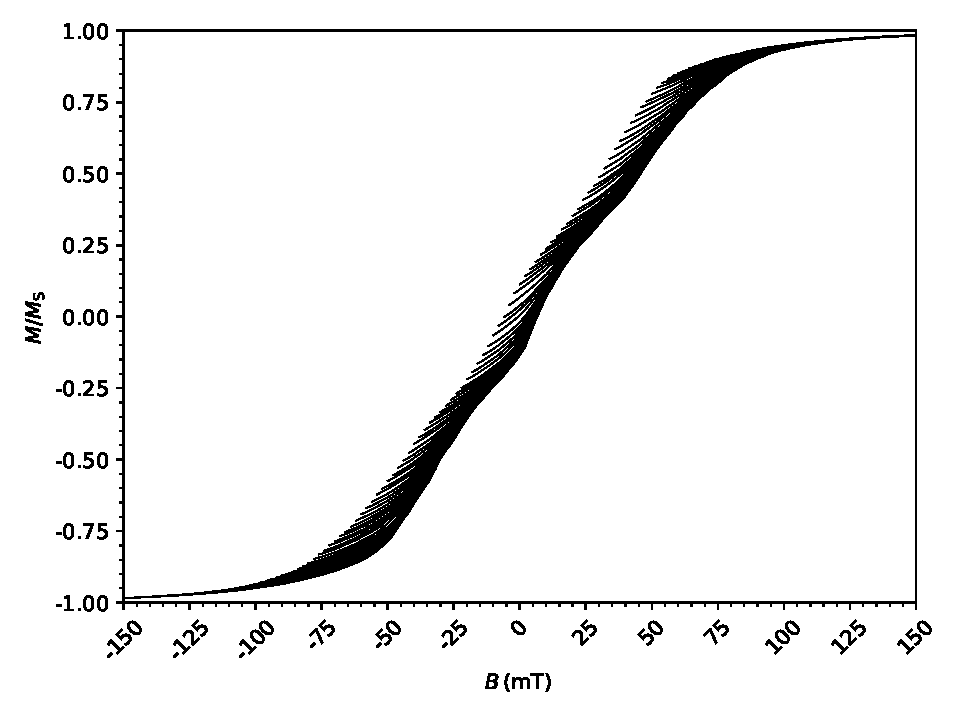
\includegraphics[width=\textwidth]{research-4/figs/BM_fram_avg.pdf}
\caption[FORCs of the framboid dispersion]{FORCs of the framboid dispersion.}
\label{FIG_10}
\end{figure}

\begin{figure}
\centering
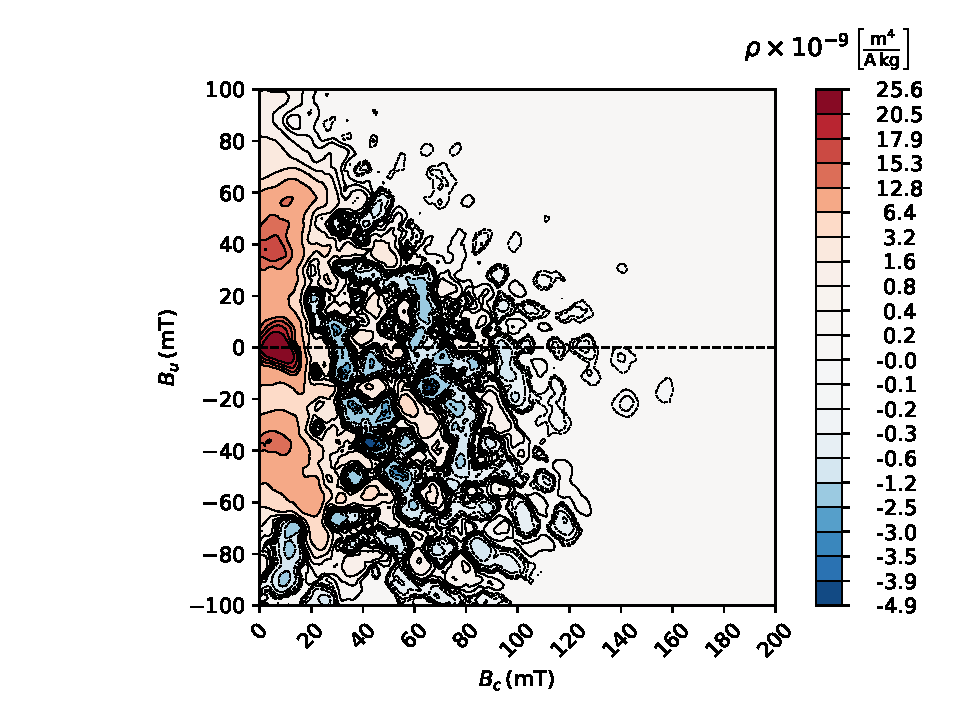
\includegraphics[width=\textwidth]{research-4/figs/FORC_framAVG_SF4.pdf}
\caption[FORC diagram of the framboid dispersion]{FORC diagram (SF=4) of the framboid dispersion.}
\label{FIG_11}
\end{figure}

\begin{figure}
\centering
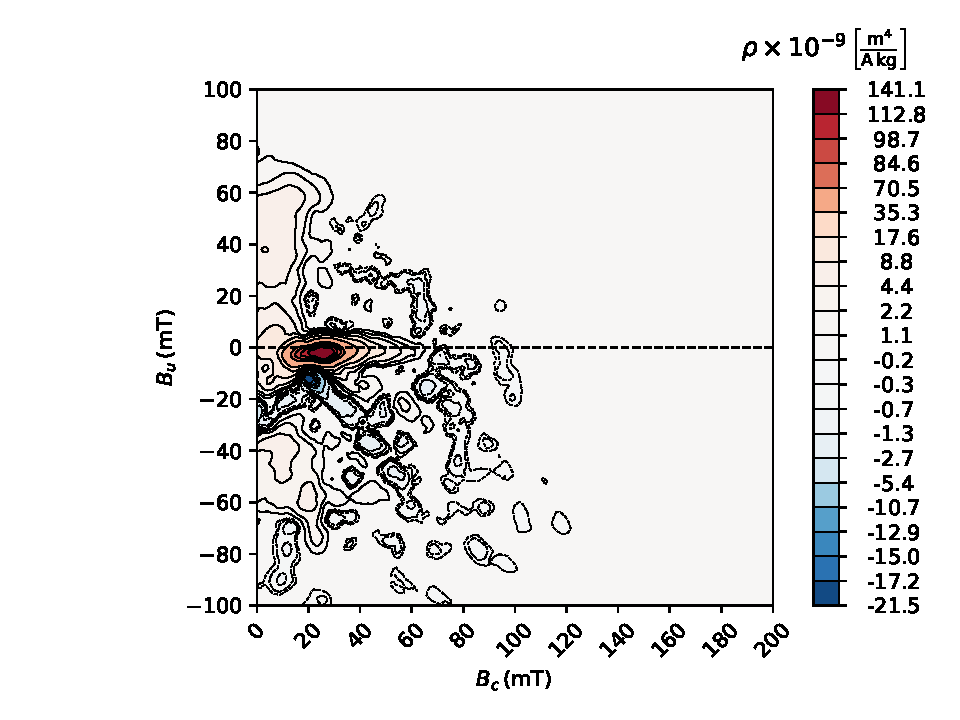
\includegraphics[width=\textwidth]{research-4/figs/FORC_framAVG_SF4_mixed_SD_ratio1.pdf}
\caption[FORCs of a dispersion of framboids and noninteracting SD particles]{FORCs of a dispersion of framboids and noninteracting particles.}
\label{FIG_12}
\end{figure}

\begin{figure}
\centering
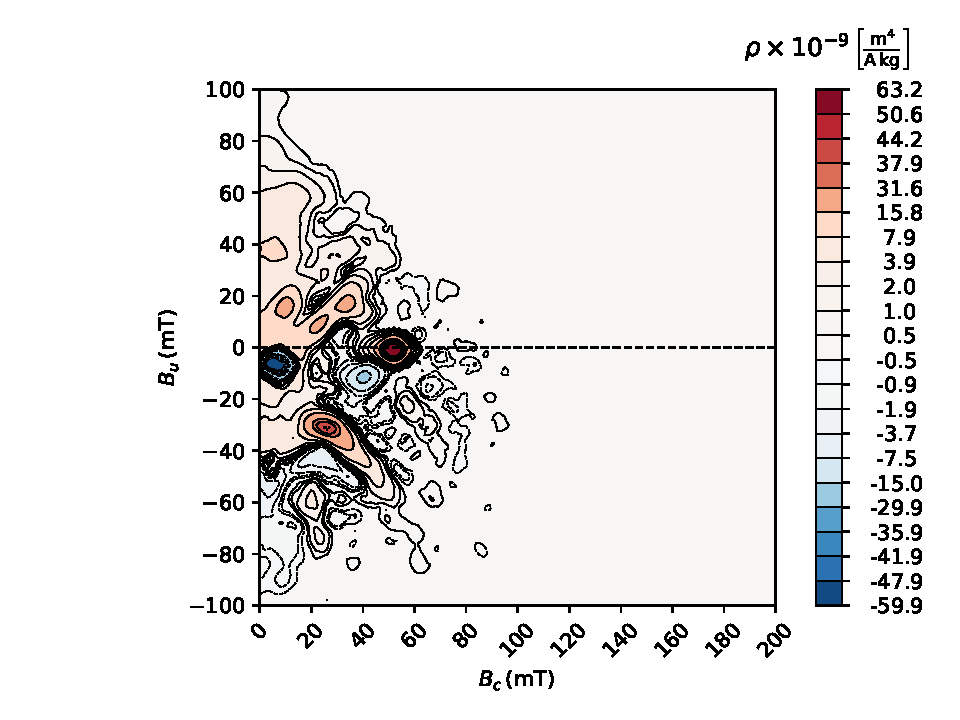
\includegraphics[width=\textwidth]{research-4/figs/FORC_framAVG_SF4_mixed_vortex_ratio1.pdf}
\caption[FORCs of a dispersion of framboids and noninteracting SV particles]{FORCs of a dispersion of framboids and noninteracting SV particles.}
\label{FIG_13}
\end{figure}

\begin{figure}
\centering
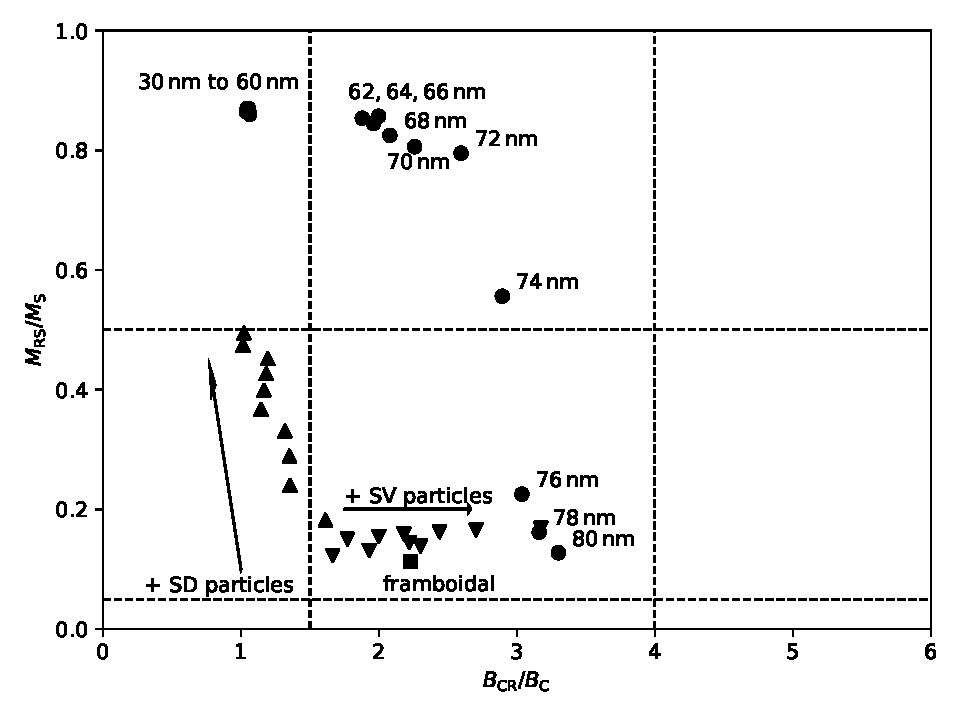
\includegraphics[width=\textwidth]{research-4/figs/DayPlot.pdf}
\caption[Day plot of framboid and noninteraring particles mixtures]{Day plot of framboid and noninteraring particles mixtures.}
\label{FIG_14}
\end{figure}

\subsection{Remanent states}
The remanent states, micromagnetic solutions and electron holography maps. Explain about the remanent states and how they would appear under electron holography studies. Important to stress how the electron holography maps can be misleading as evidenced by Figs. \ref{FIG_21}, \ref{FIG_22}, \ref{FIG_23}, \ref{FIG_24}, \ref{FIG_25}, \ref{FIG_26} which show either a single-vortex or a two-vortex structure depending on the angle of the beam.\par
\begin{figure}
\centering
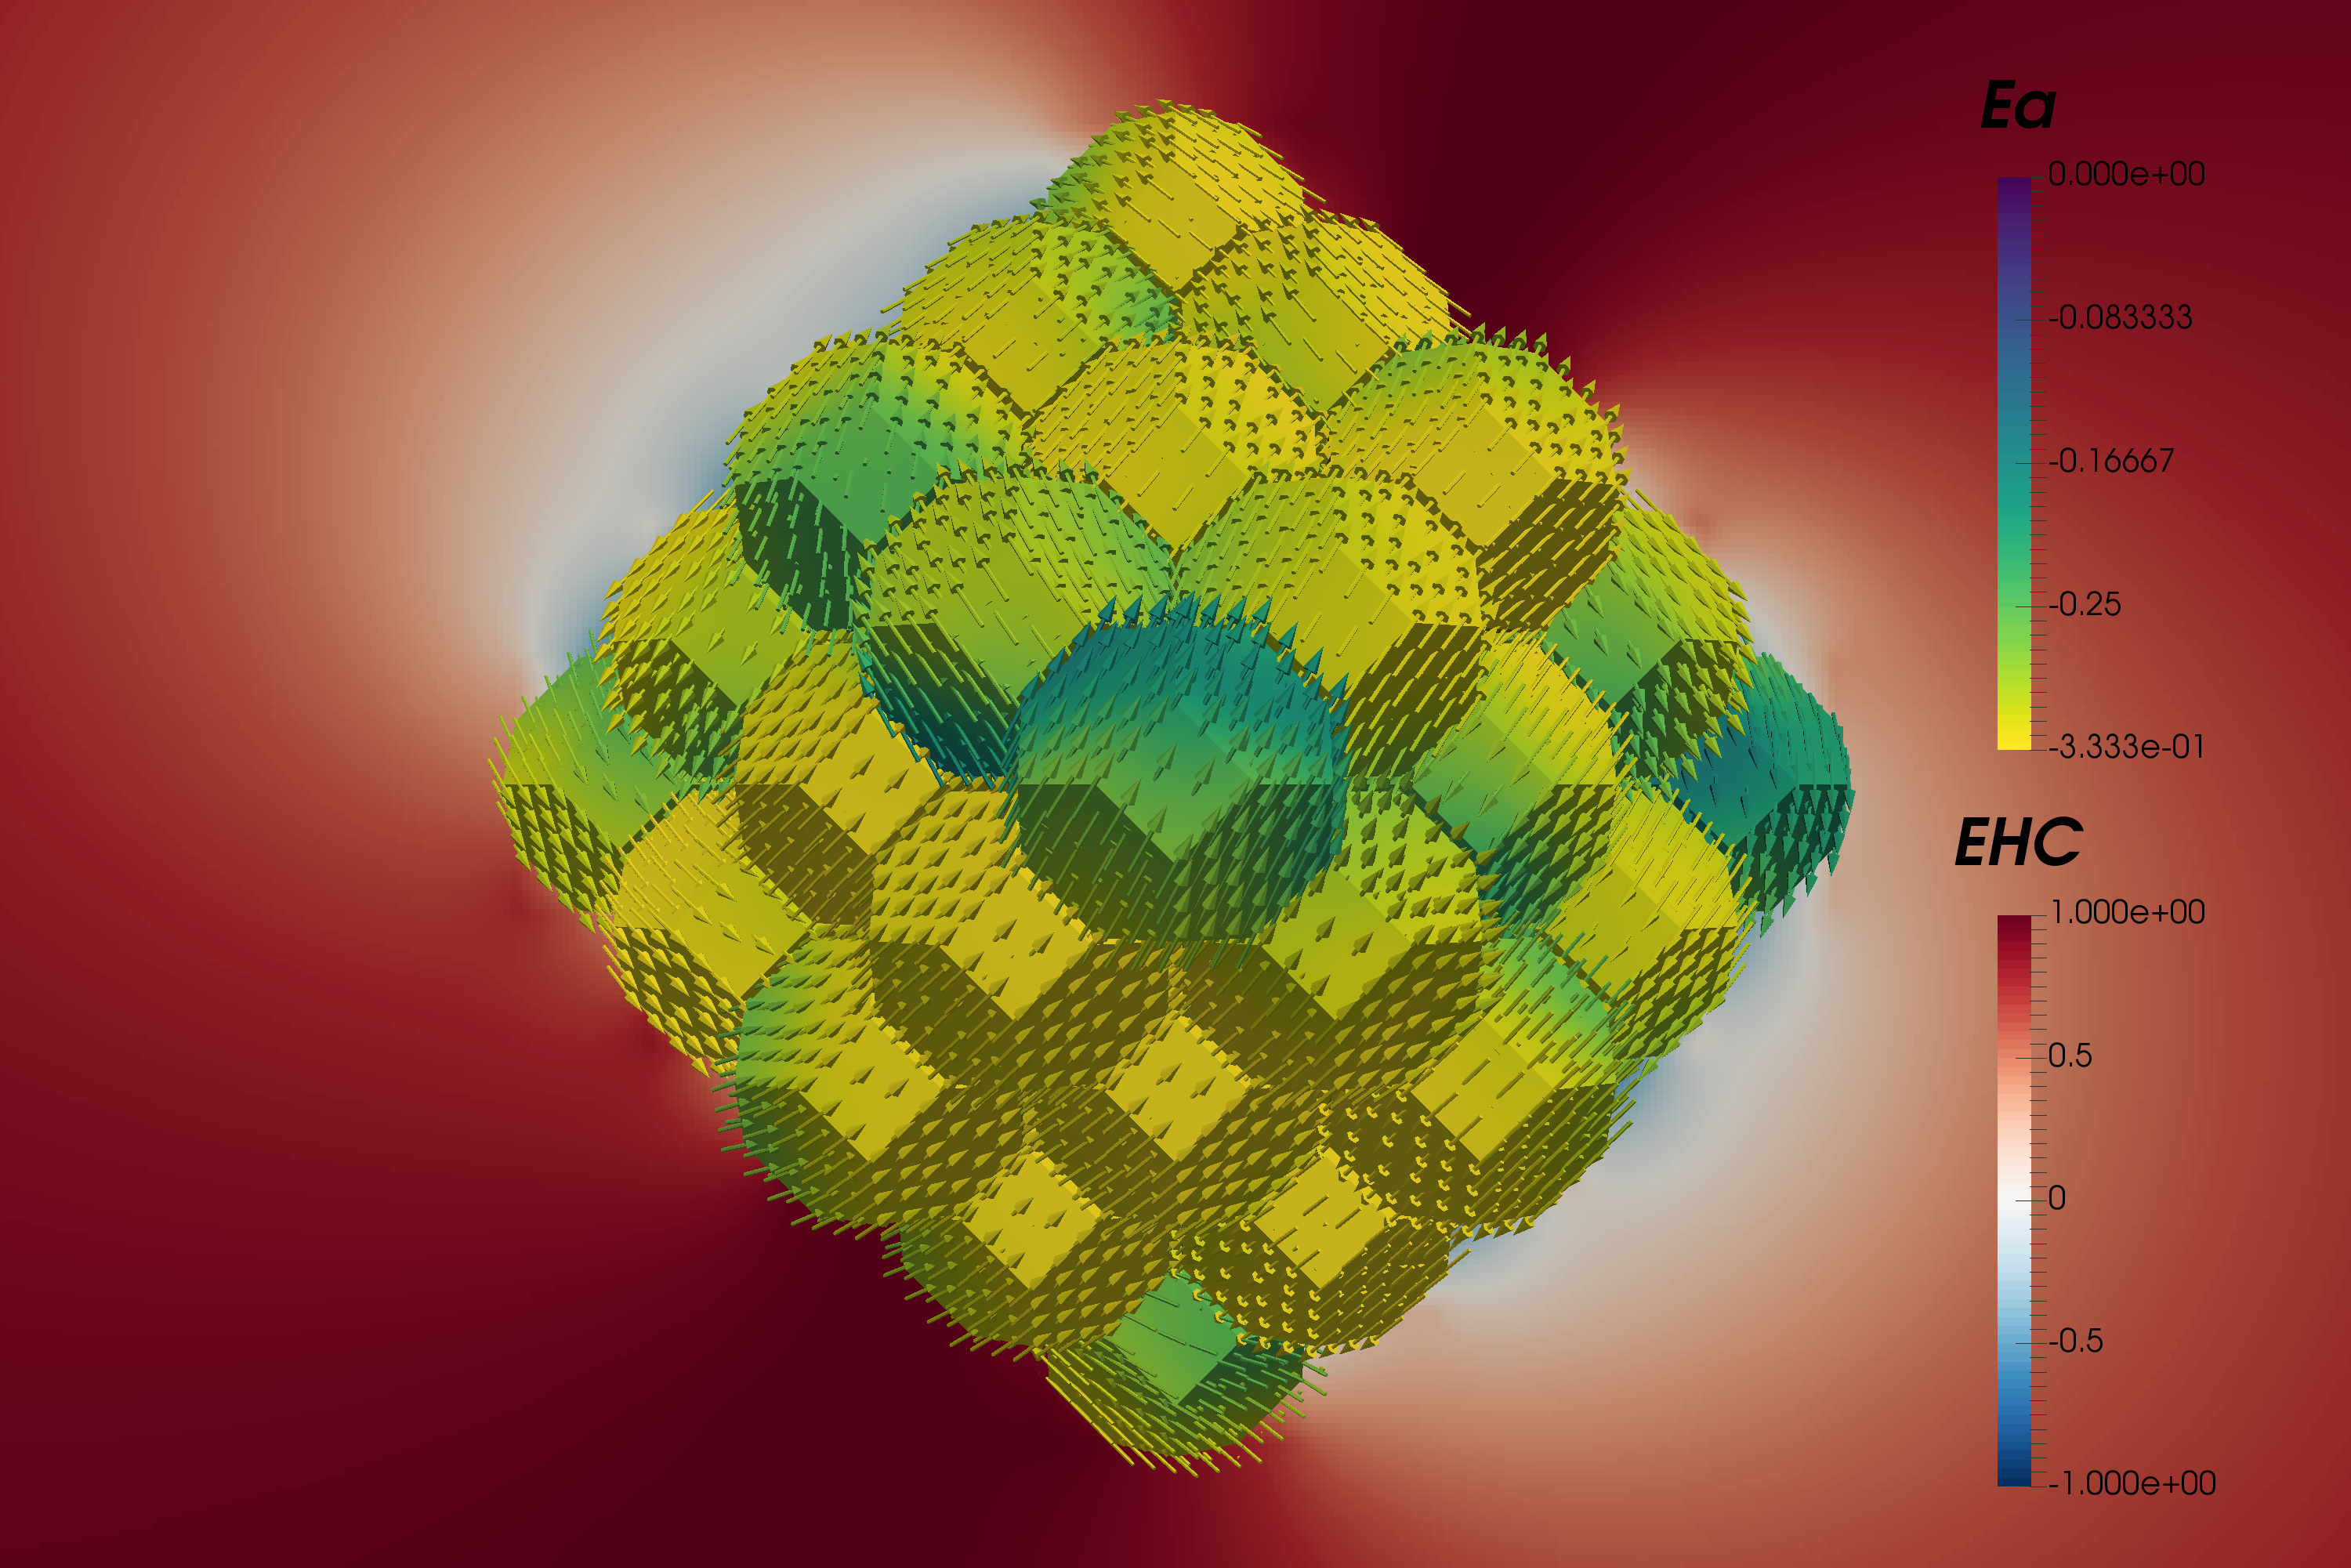
\includegraphics[width=\textwidth]{research-4/figs/fram_i21_f0_-z.png}
\caption[Remanent state when the field is along an easy axis (view from +Z)]{Remanent state when the field is along an easy axis (view from +Z).}
\label{FIG_15}
\end{figure}

\begin{figure}
\centering
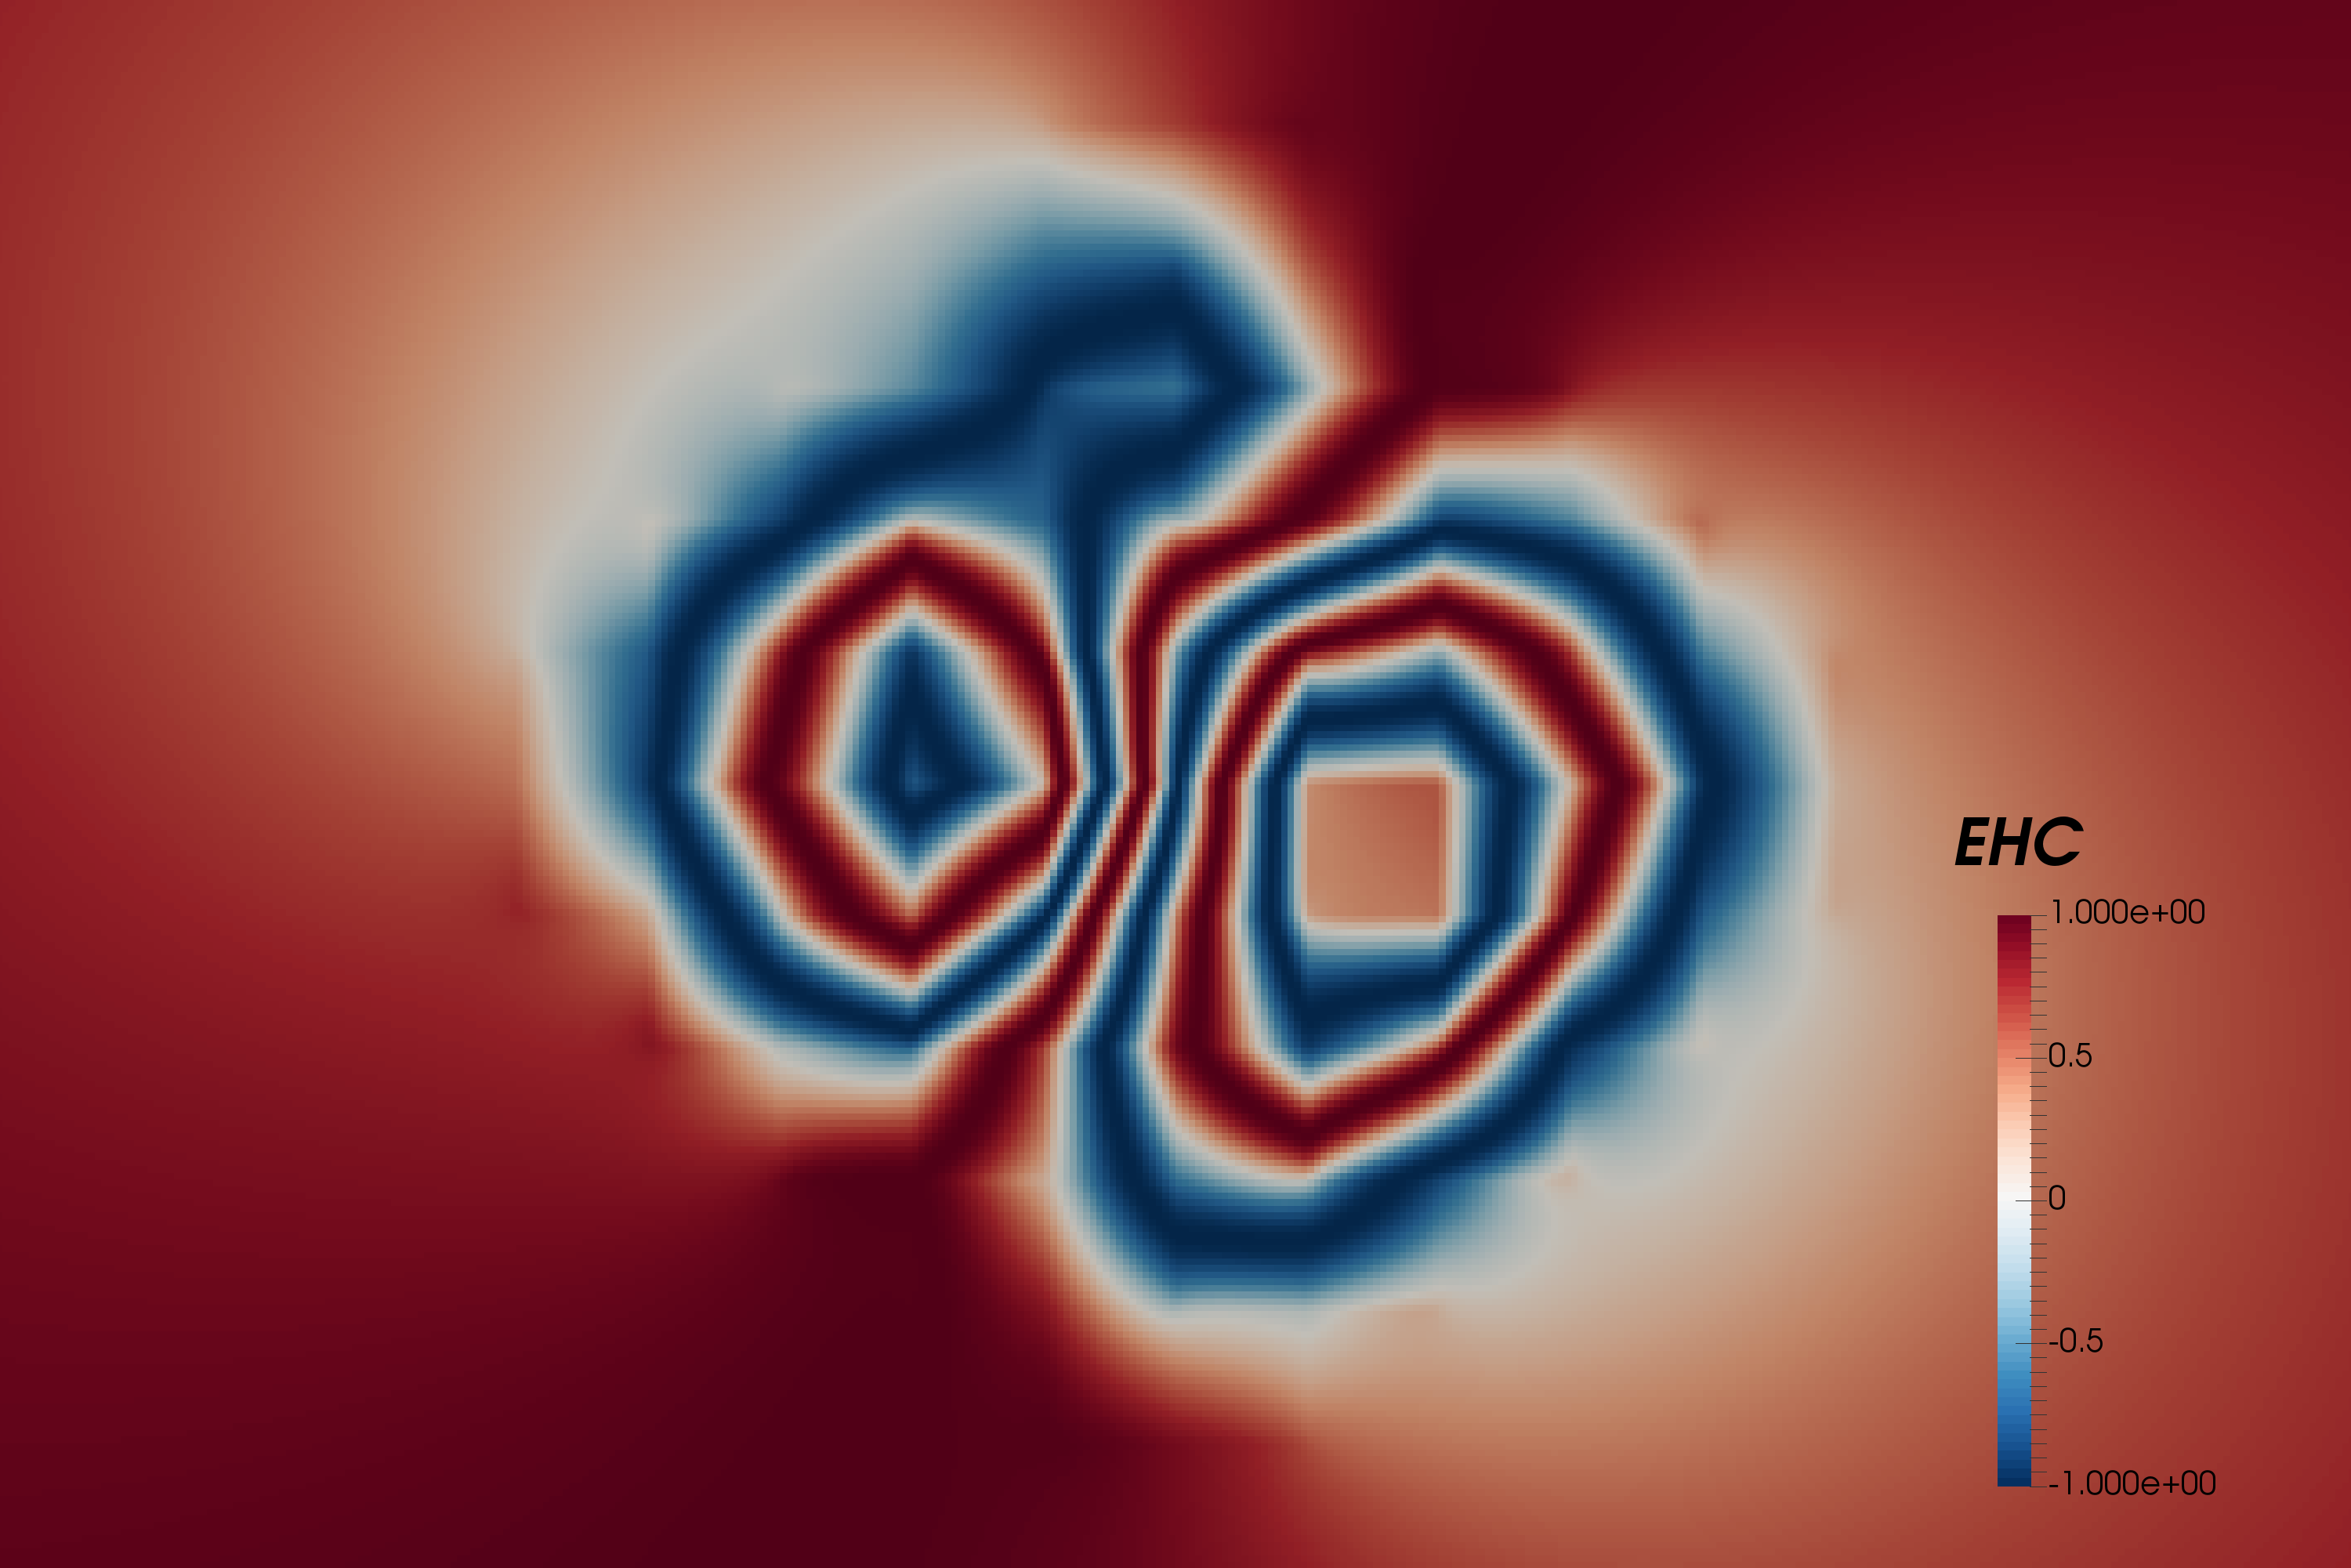
\includegraphics[width=\textwidth]{research-4/figs/fram_i21_f0_-z_EHC.png}
\caption[Electron holography map of the remanent state when the field is along an easy axis (view from +Z)]{Electron holography map of the remanent state when the field is along an easy axis (view from +Z).}
\label{FIG_16}
\end{figure}

\begin{figure}
\centering
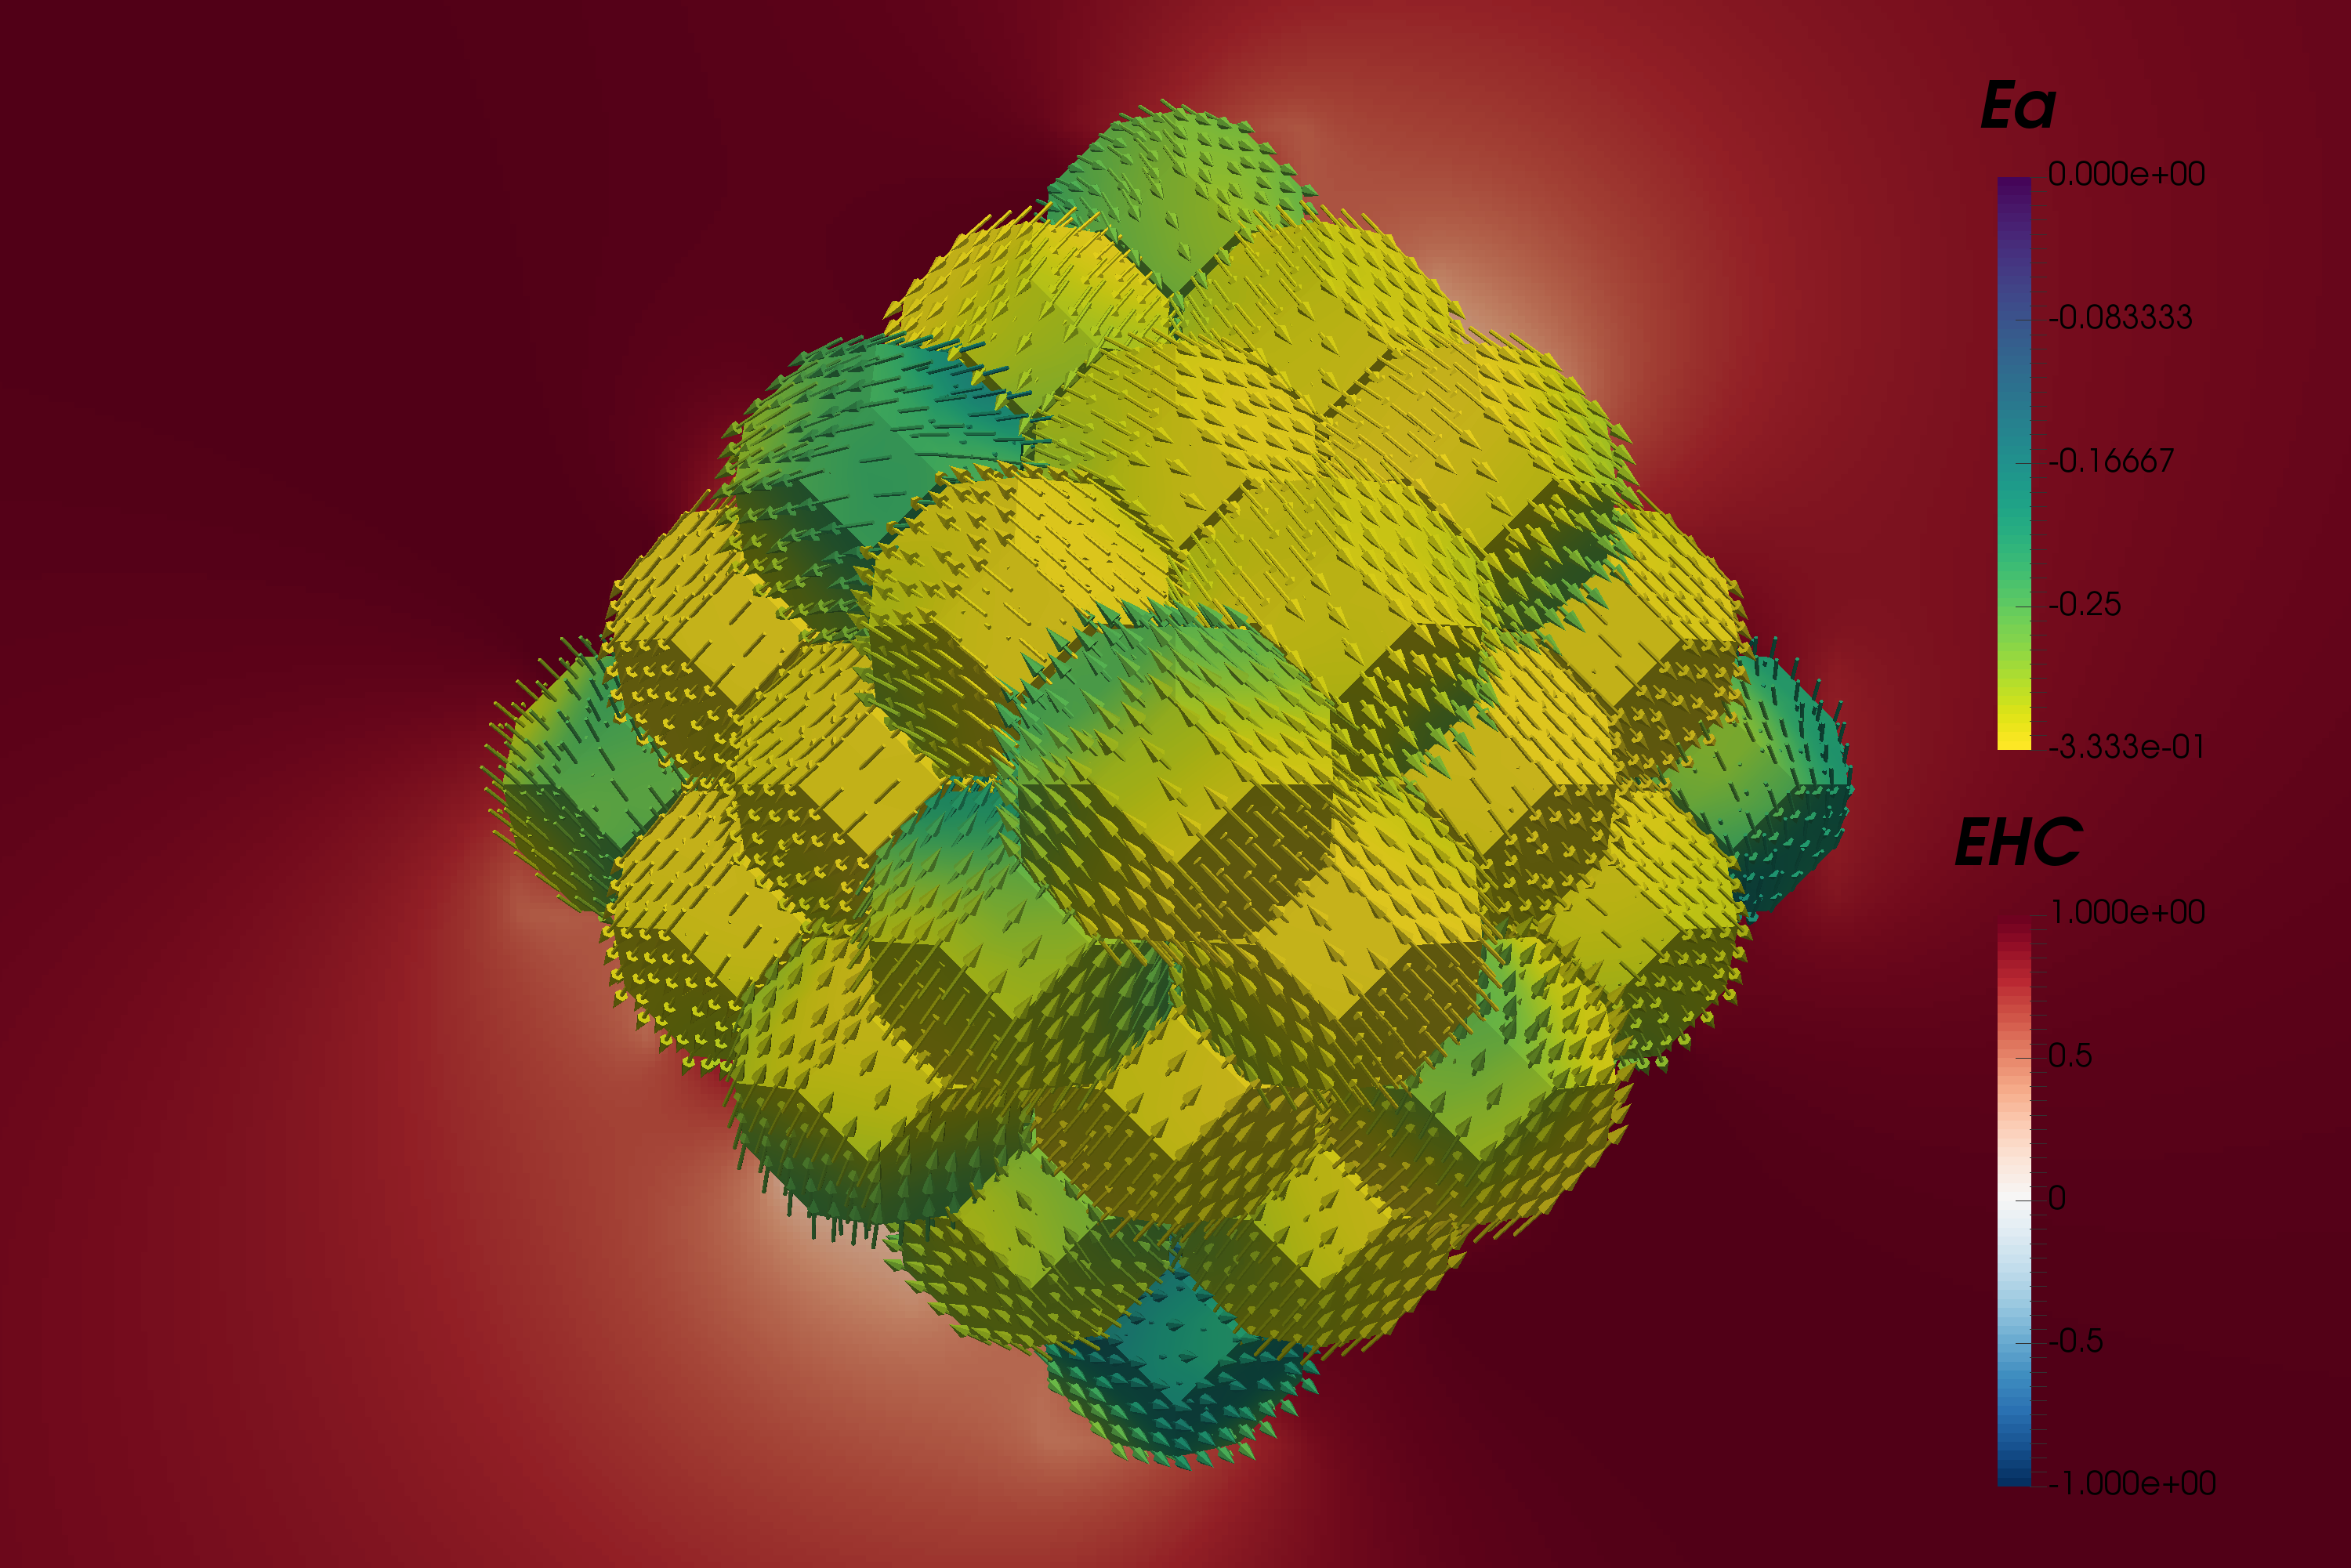
\includegraphics[width=\textwidth]{research-4/figs/fram_i21_f0_-y.png}
\caption[Remanent state when the field is along an easy axis (view from +Y)]{Remanent state when the field is along an easy axis (view from +Y).}
\label{FIG_17}
\end{figure}

\begin{figure}
\centering
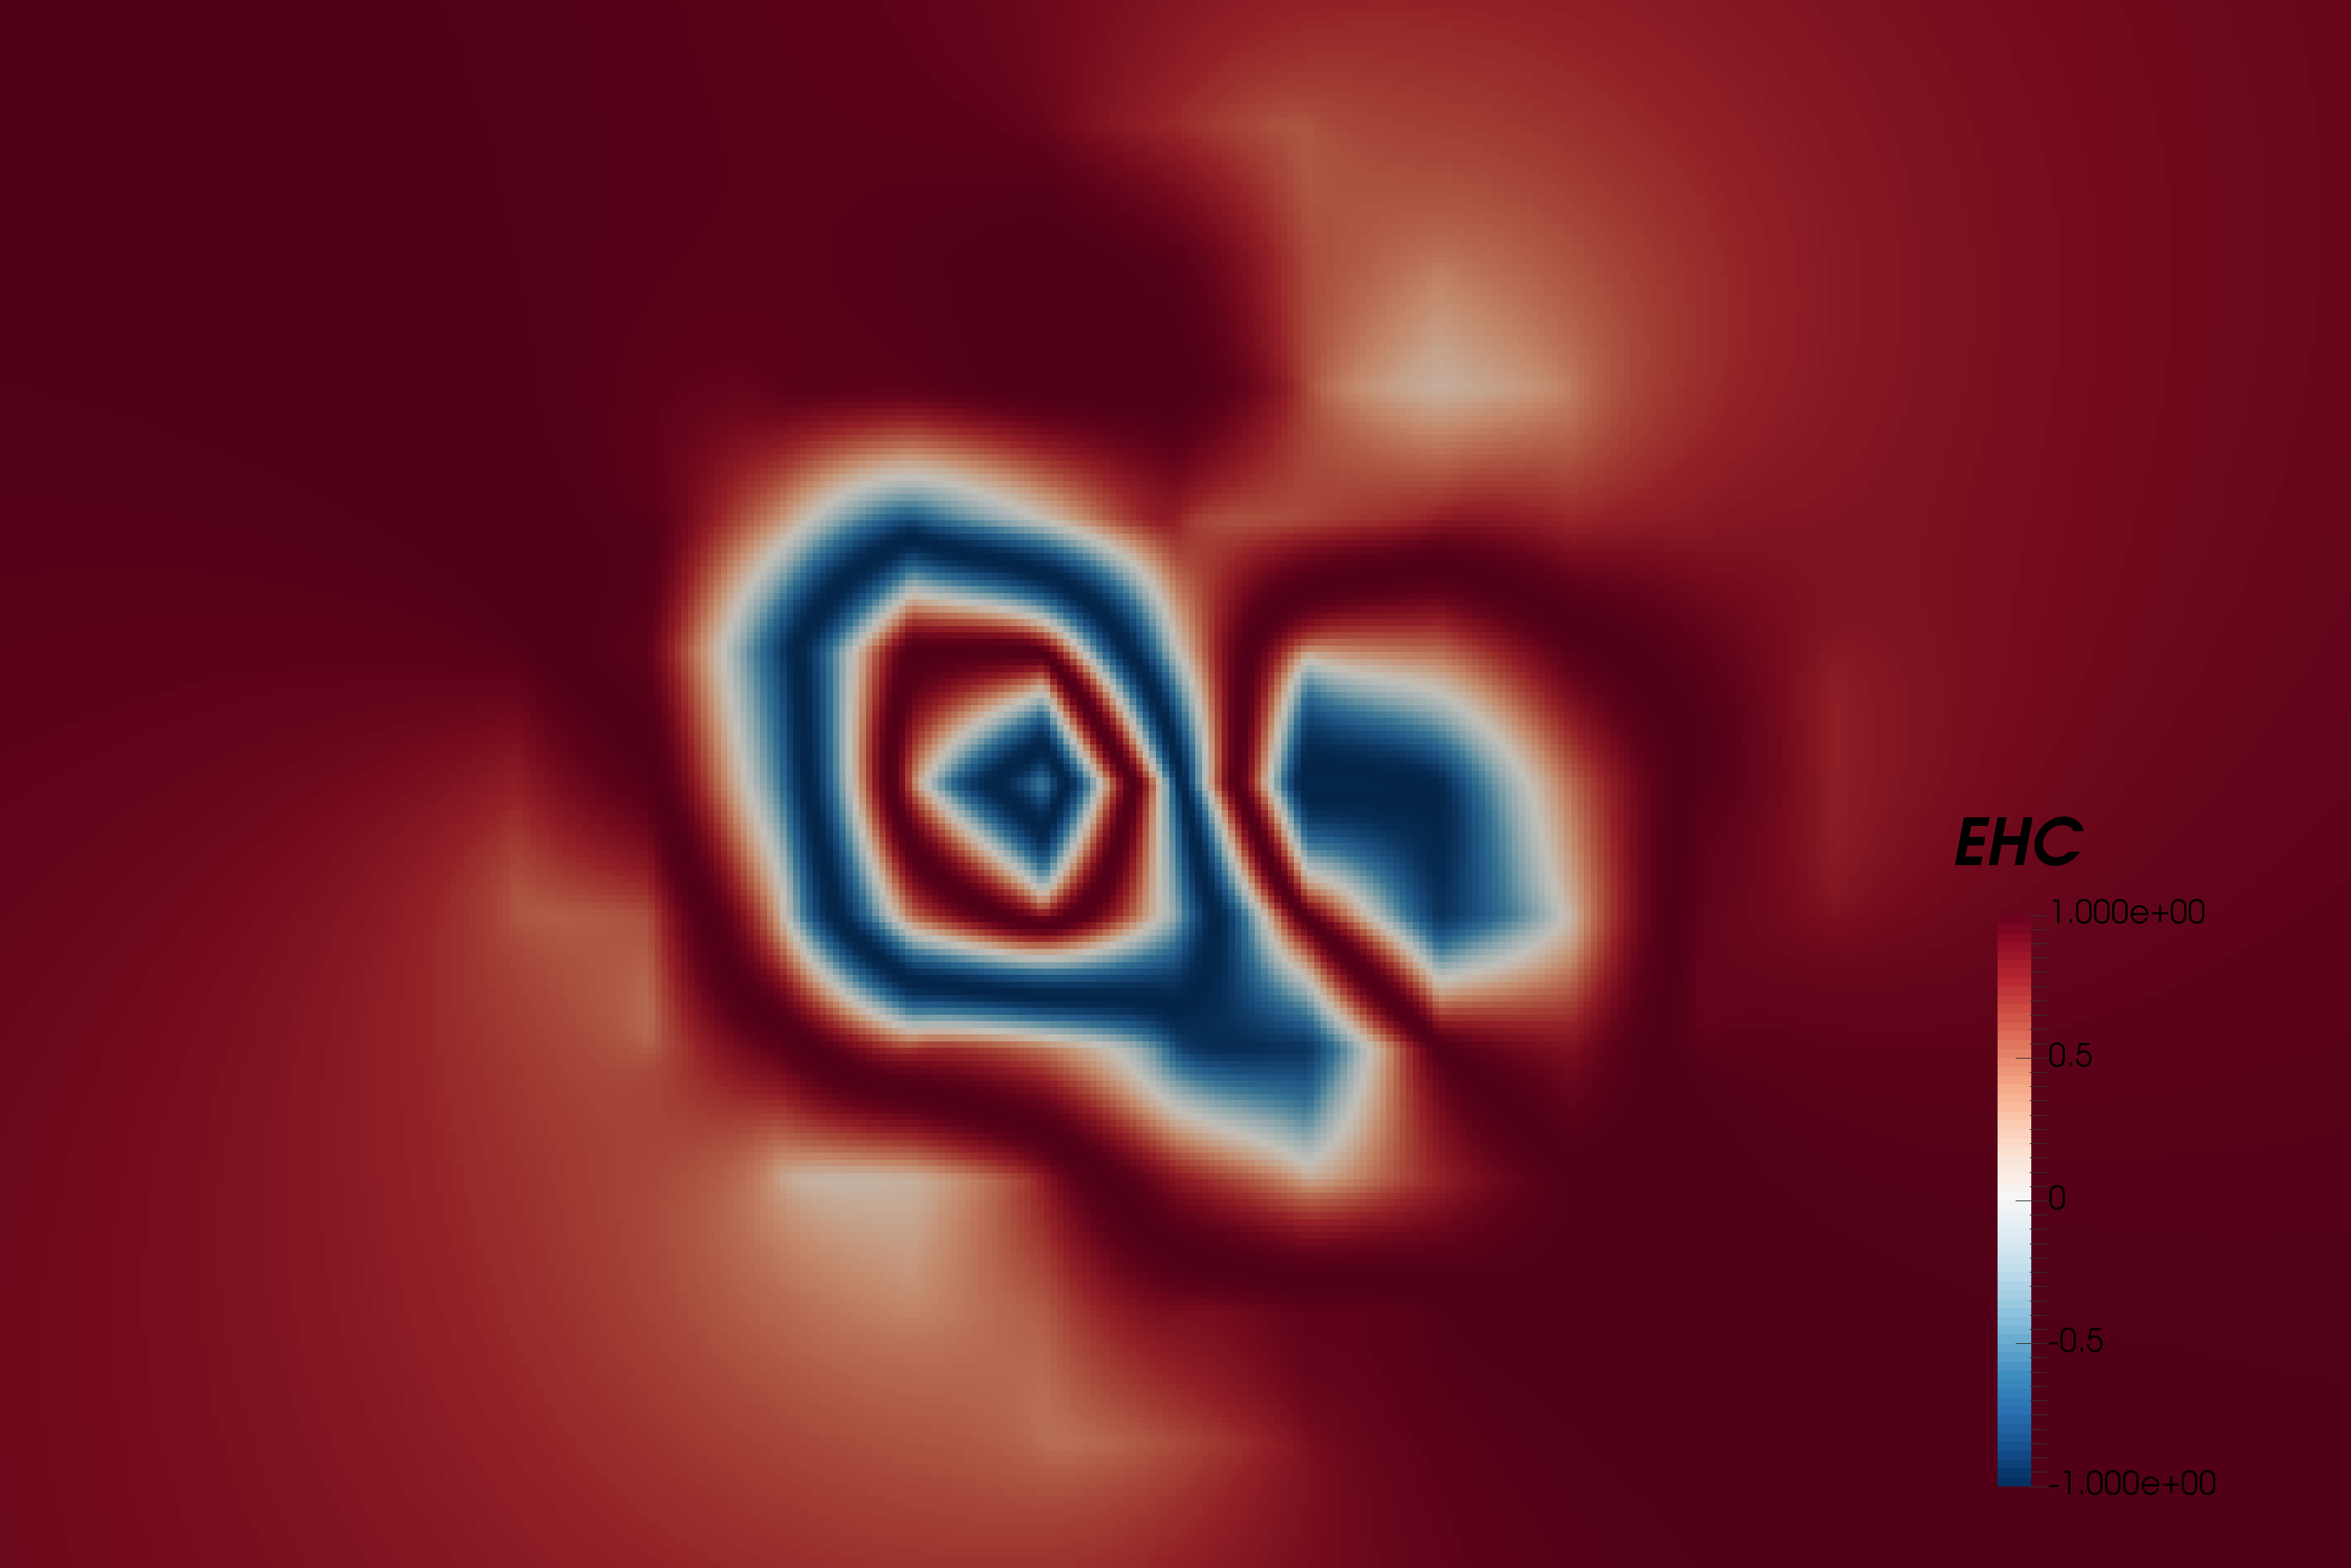
\includegraphics[width=\textwidth]{research-4/figs/fram_i21_f0_-y_EHC.png}
\caption[Electron holography map of the remanent state when the field is along an easy axis (view from +Y)]{Electron holography map of the remanent state when the field is along an easy axis (view from +Y).}
\label{FIG_18}
\end{figure}

\begin{figure}
\centering
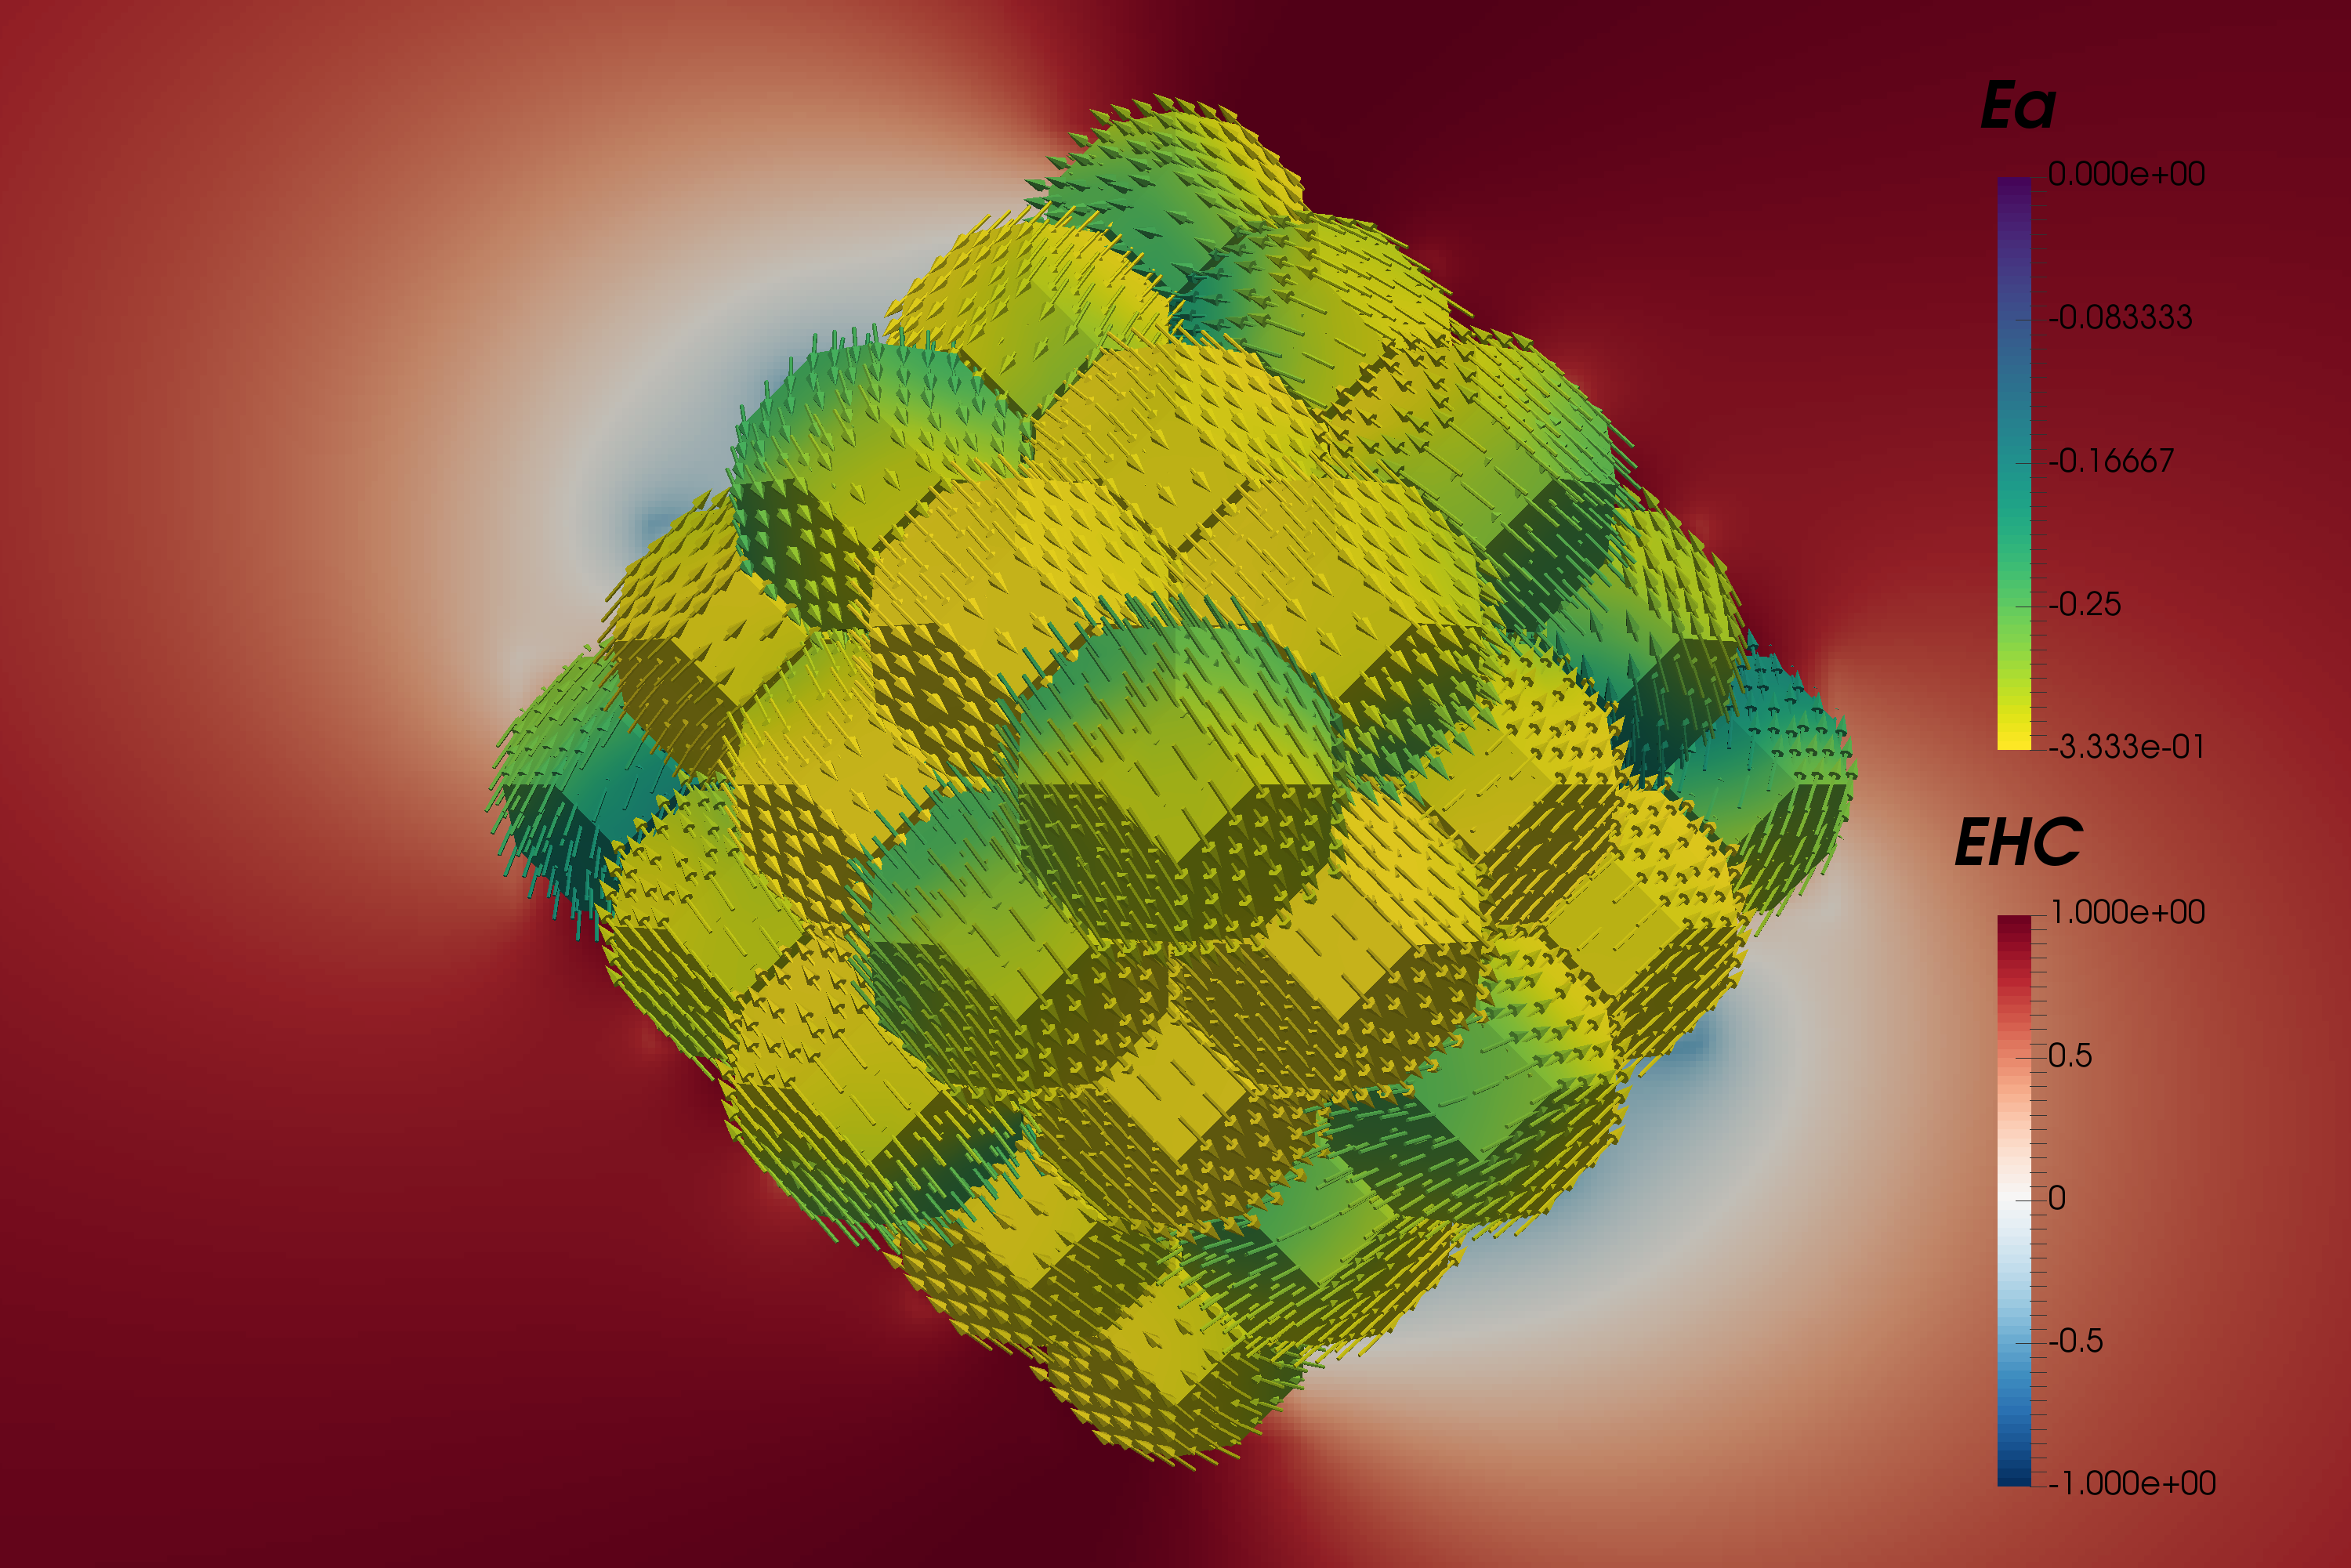
\includegraphics[width=\textwidth]{research-4/figs/fram_i21_f0_-x.png}
\caption[Remanent state when the field is along an easy axis (view from +X)]{Remanent state when the field is along an easy axis (view from +X).}
\label{FIG_19}
\end{figure}

\begin{figure}
\centering
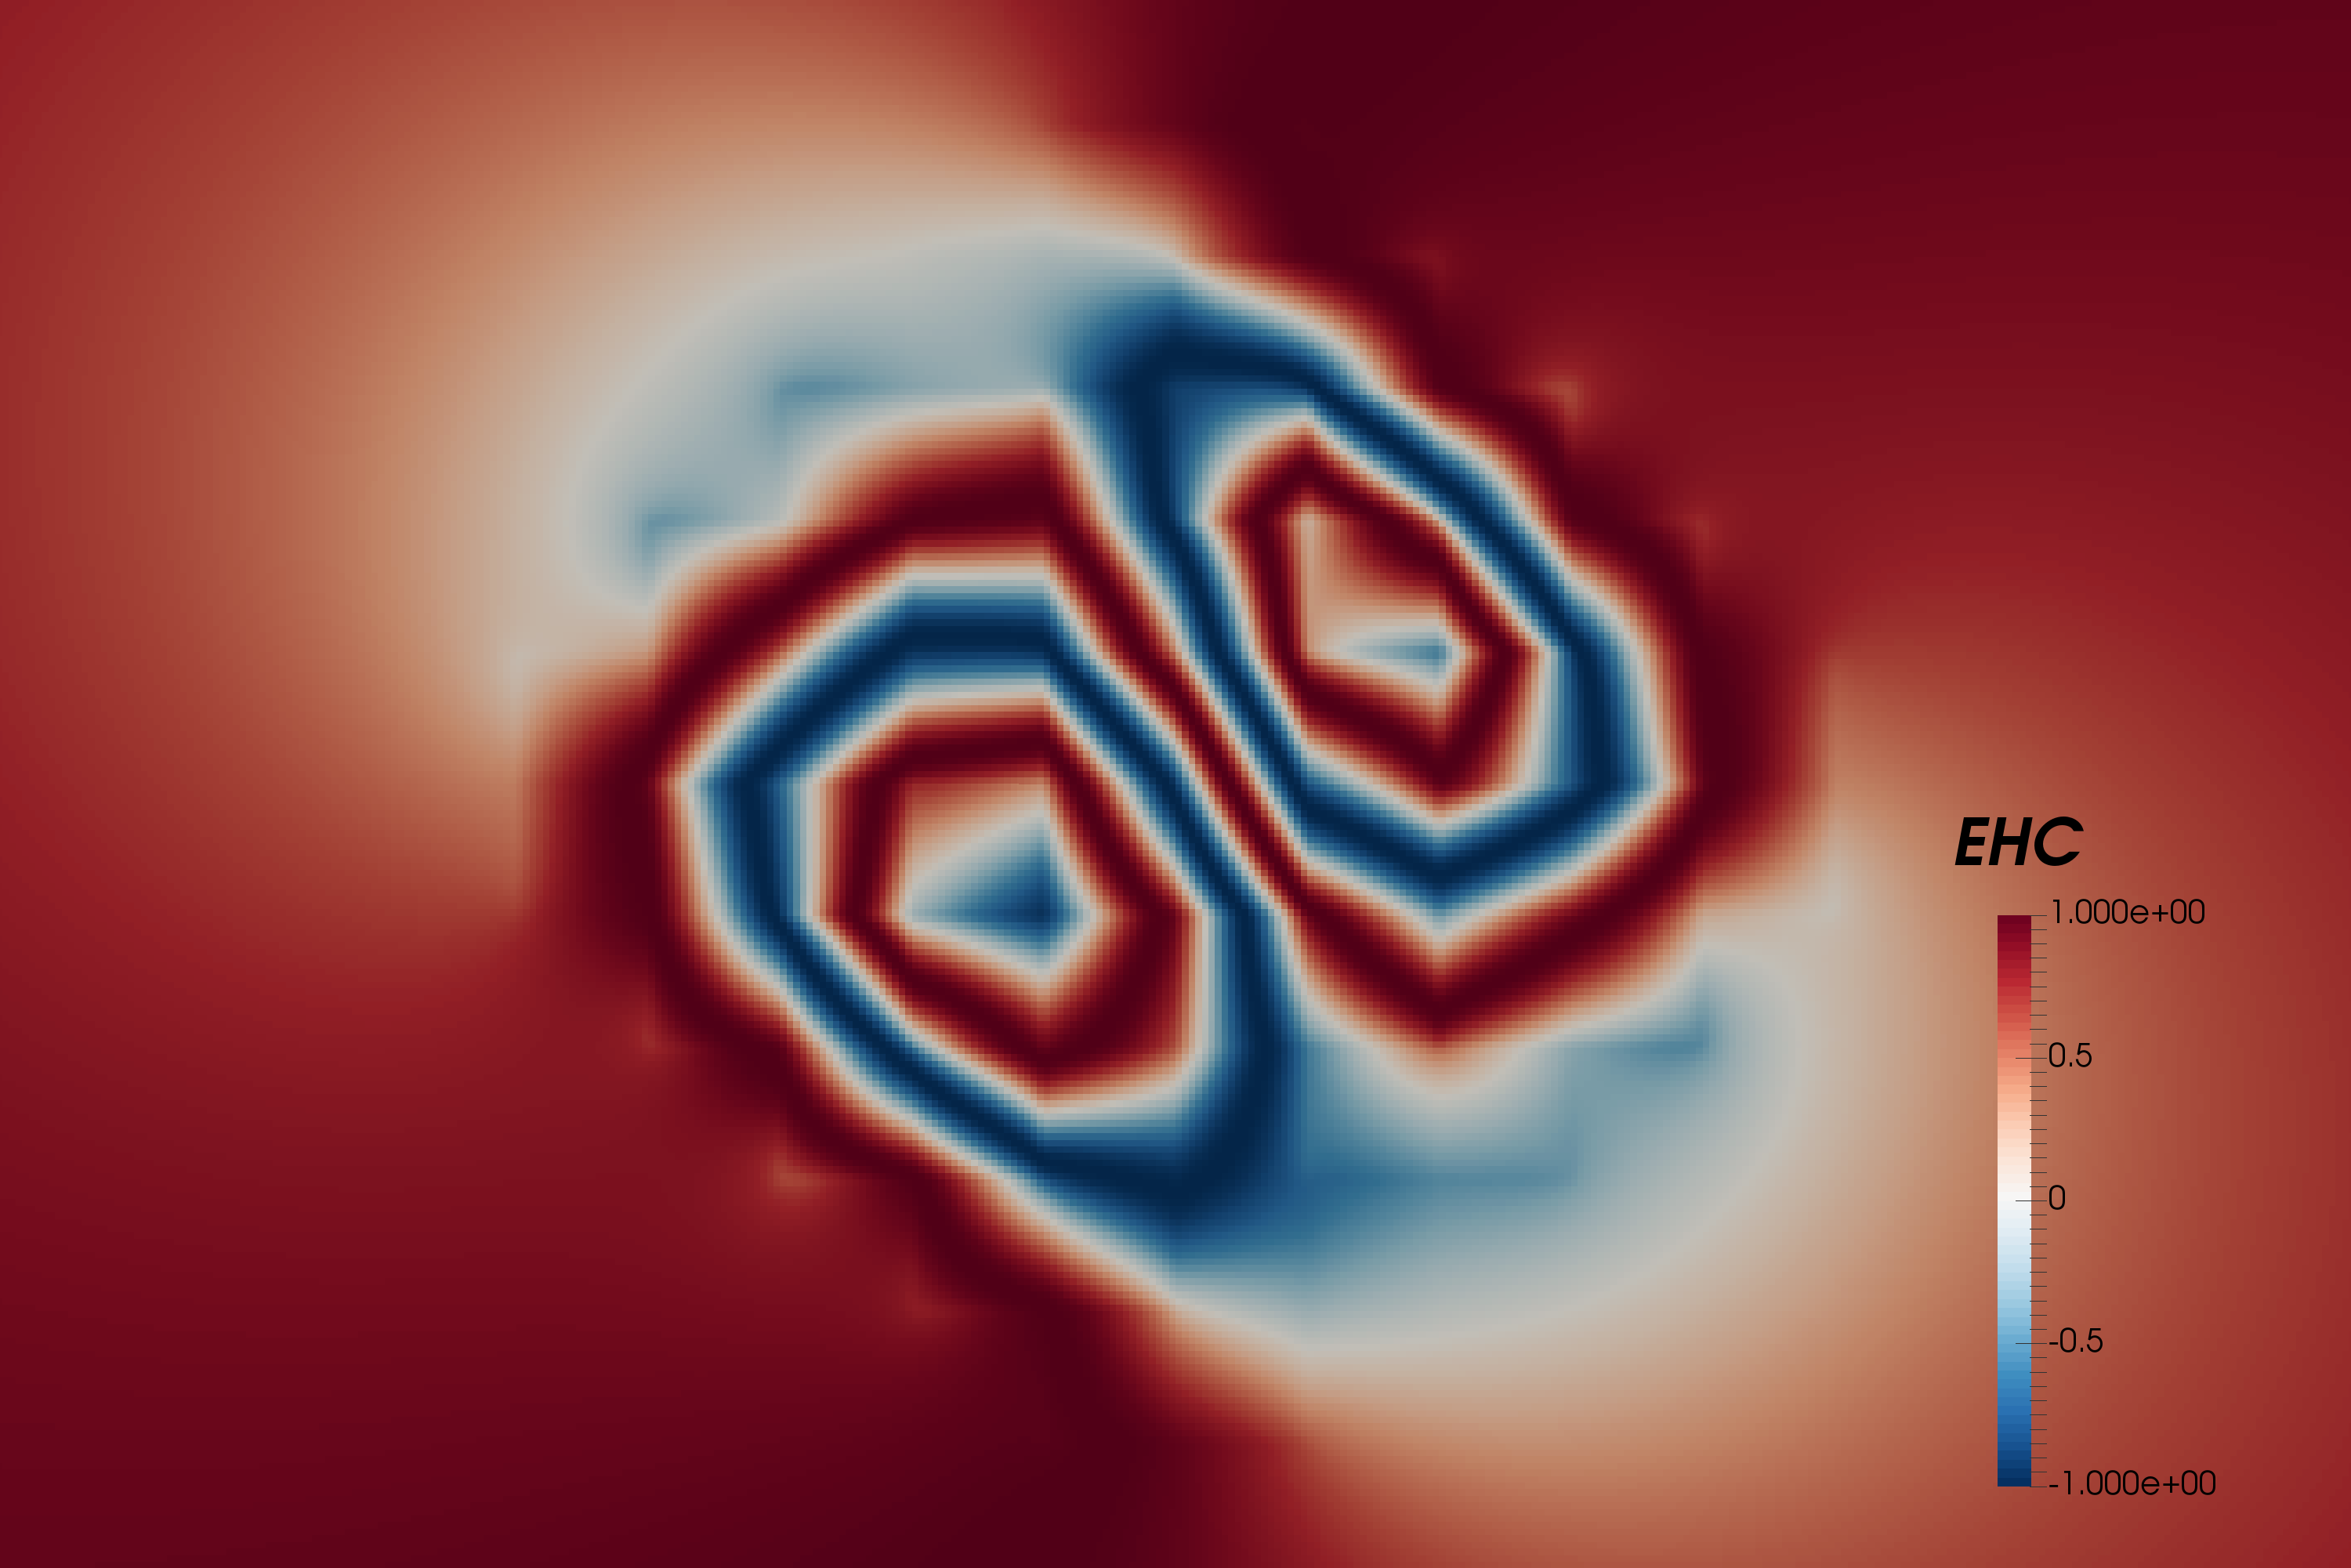
\includegraphics[width=\textwidth]{research-4/figs/fram_i21_f0_-x_EHC.png}
\caption[Electron holography map of the remanent state when the field is along an easy axis (view from +X)]{Electron holography map of the remanent state when the field is along an easy axis (view from +X).}
\label{FIG_20}
\end{figure}

\begin{figure}
\centering
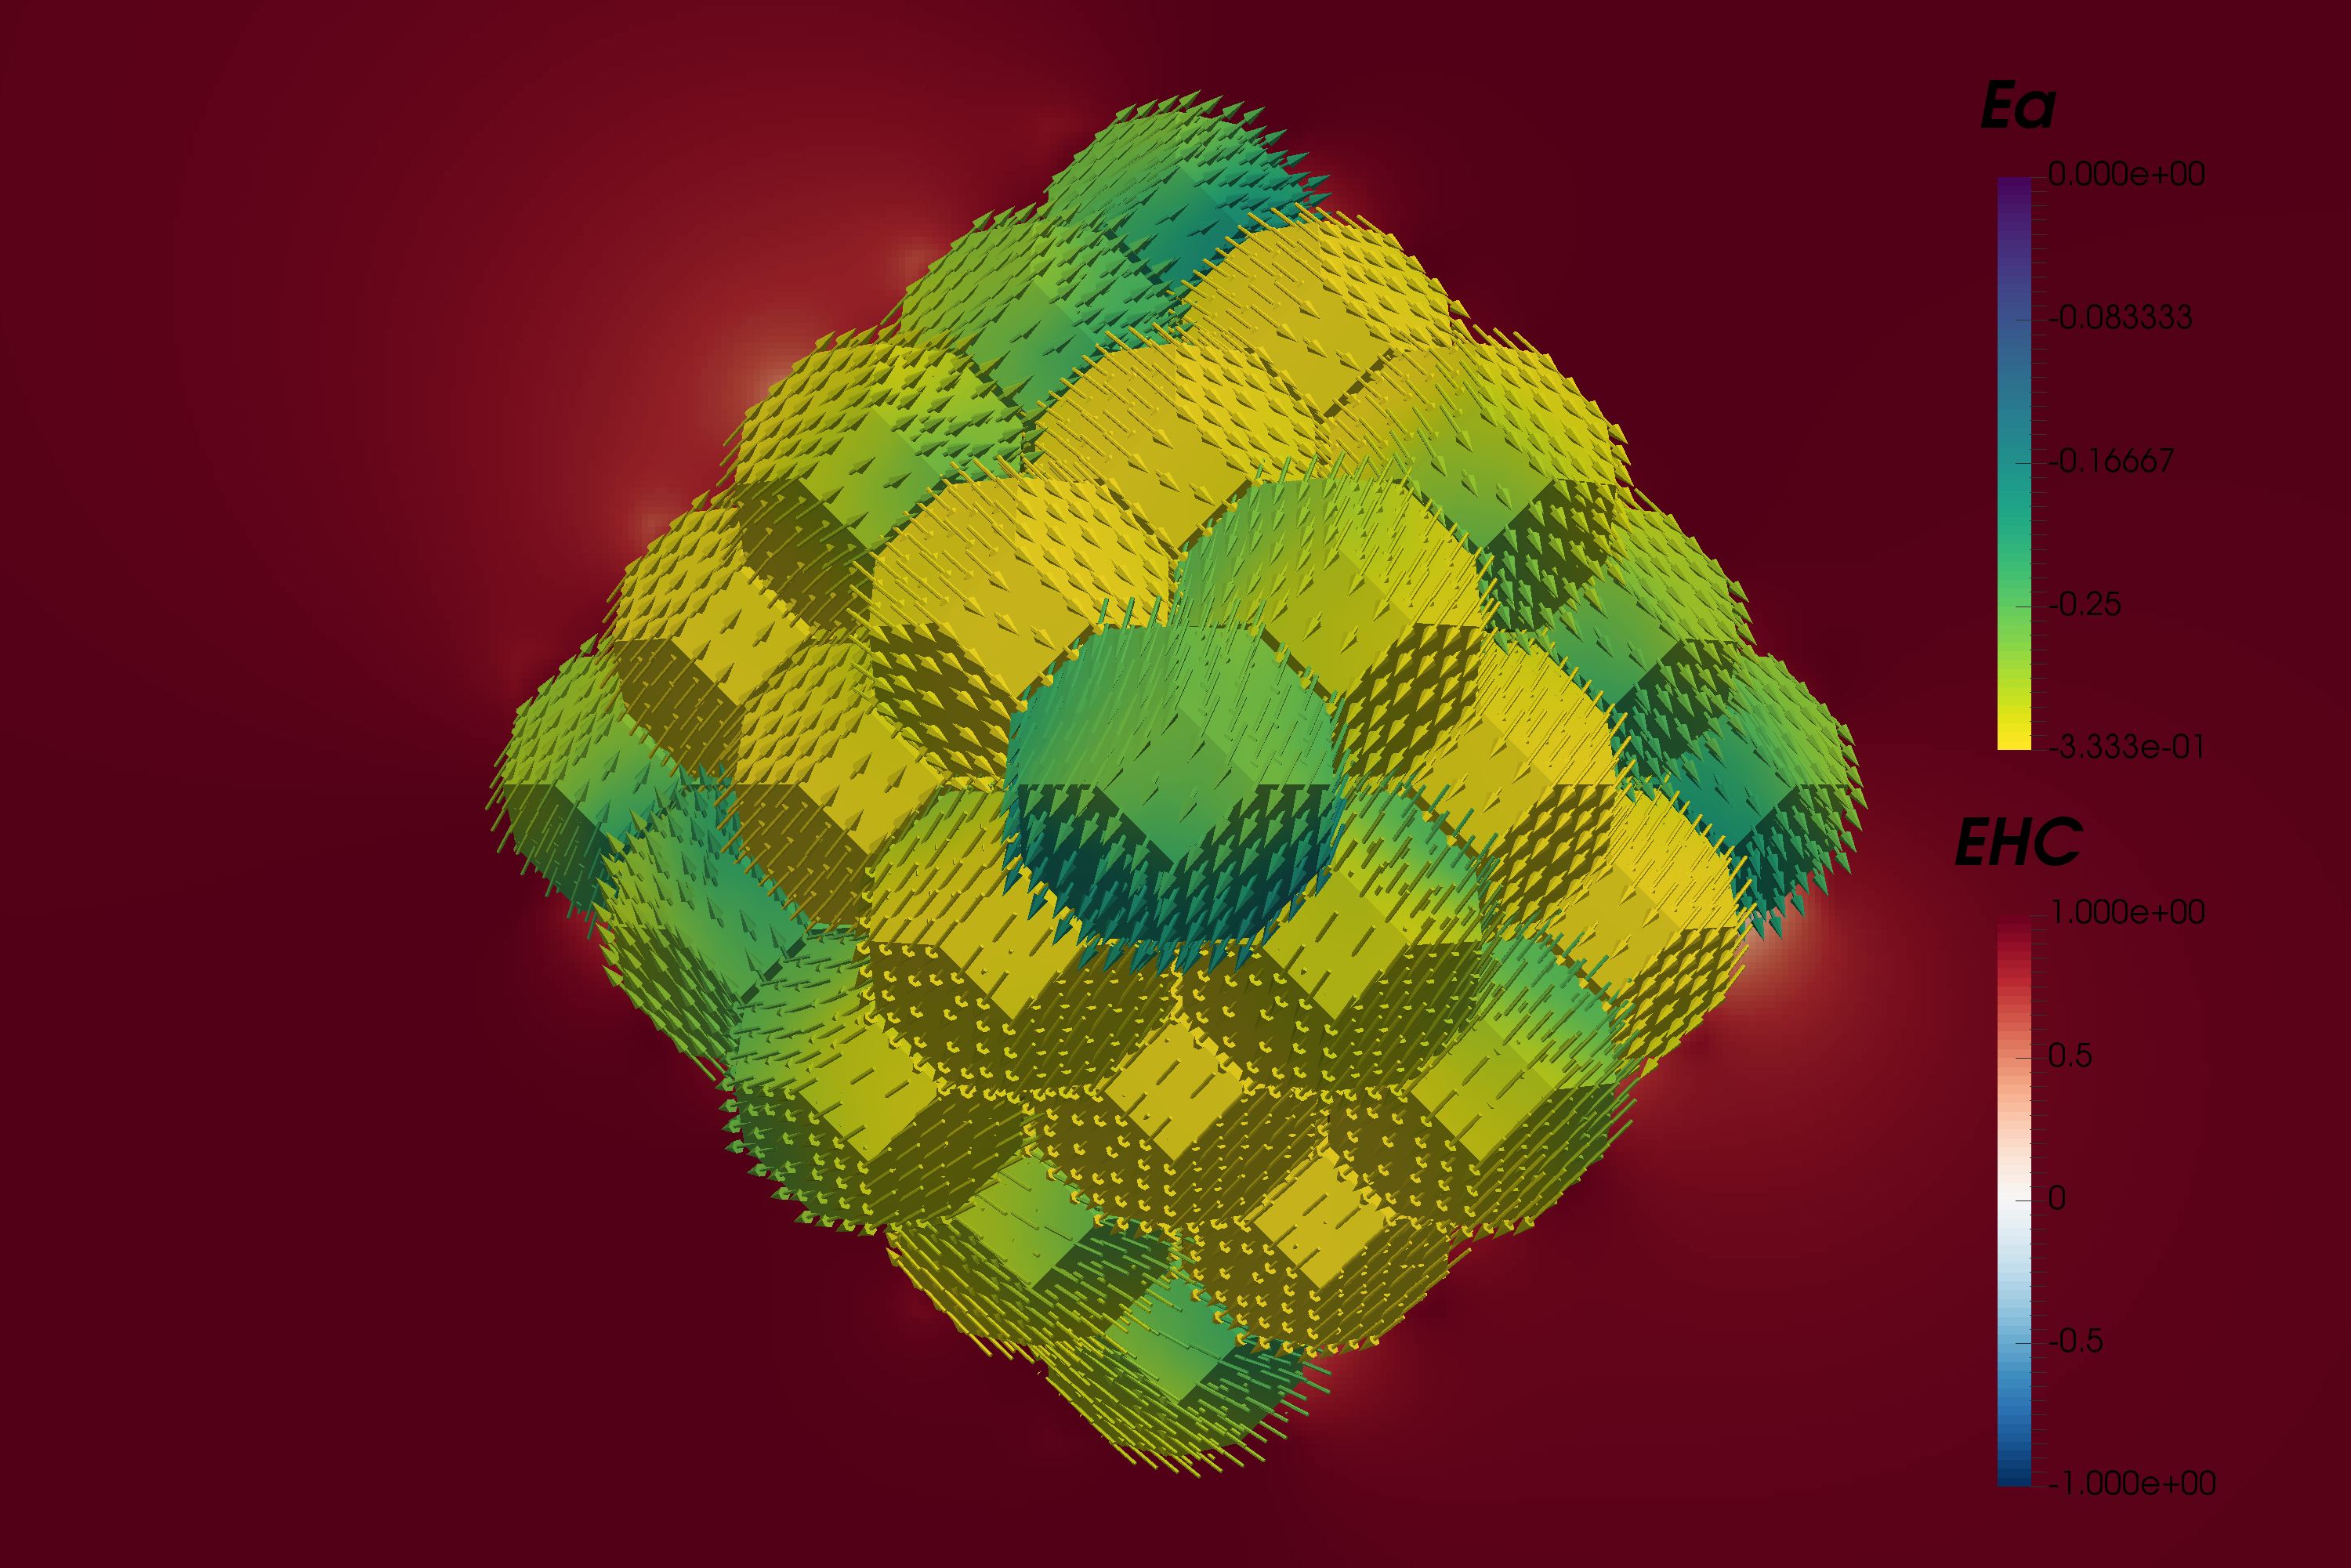
\includegraphics[width=\textwidth]{research-4/figs/fram_i16_f0_-z.png}
\caption[Remanent state when the field is along a hard axis (view from +Z)]{Remanent state when the field is along a hard axis (view from +Z).}
\label{FIG_21}
\end{figure}

\begin{figure}
\centering
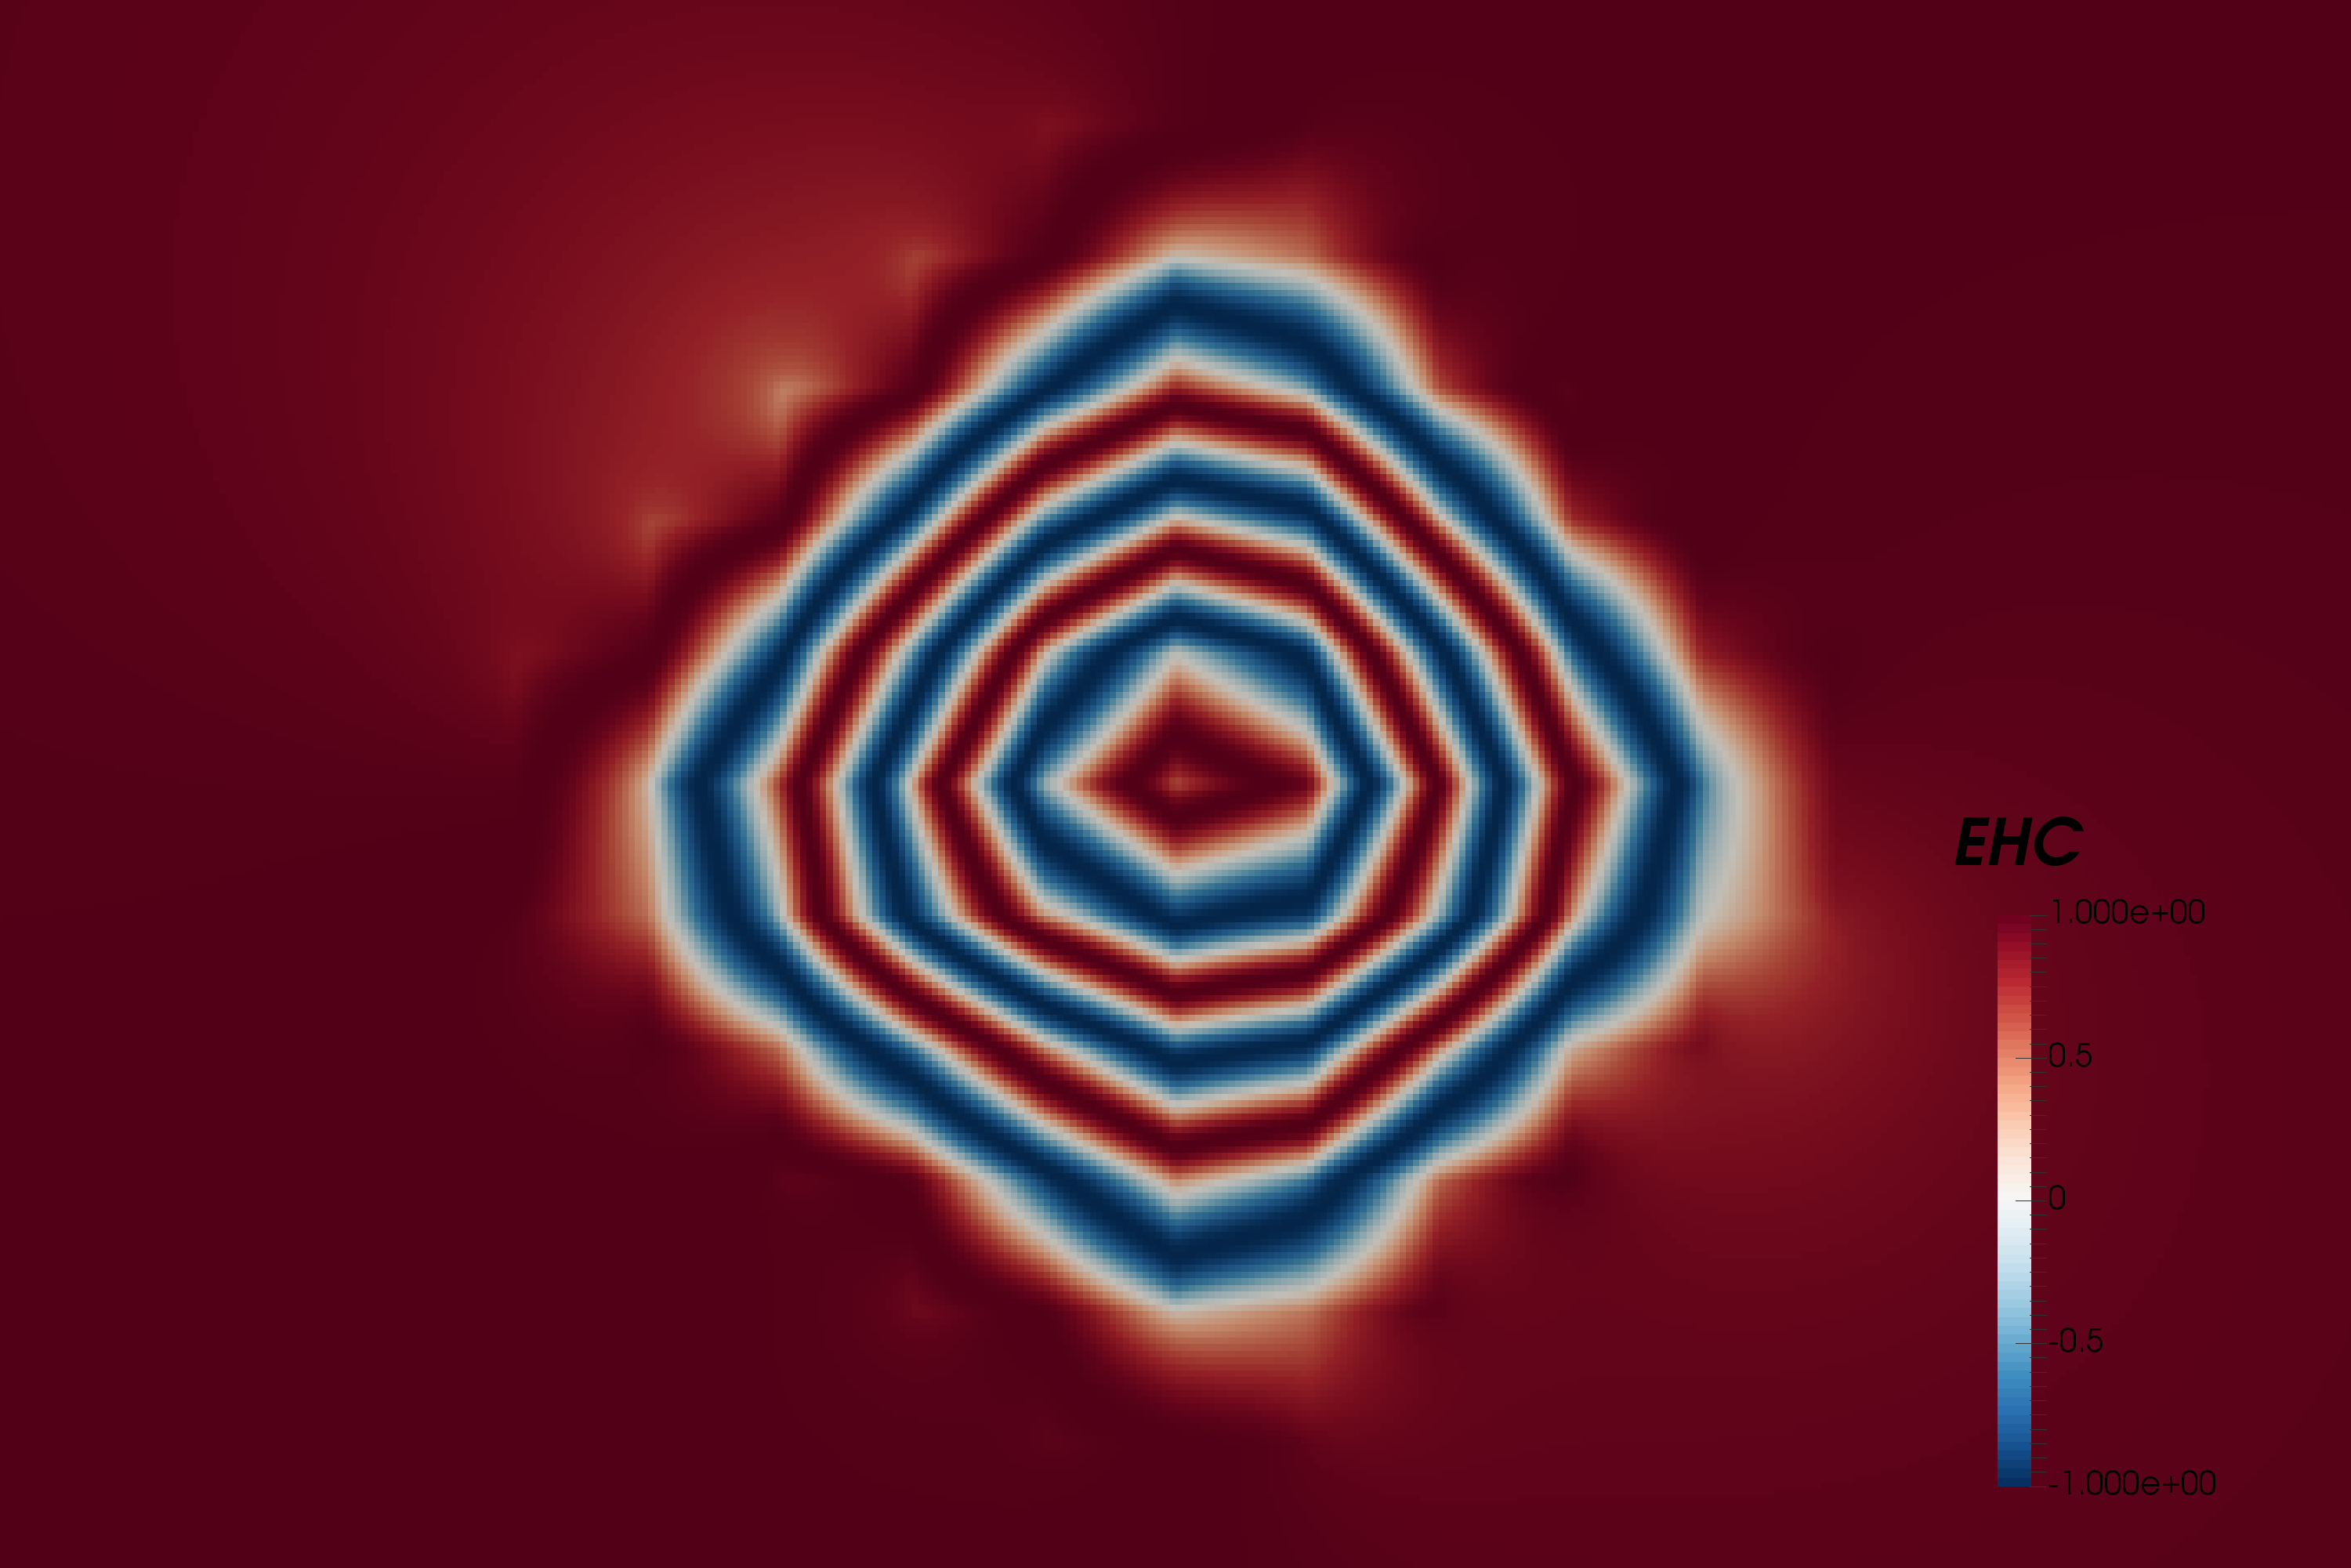
\includegraphics[width=\textwidth]{research-4/figs/fram_i16_f0_-z_EHC.png}
\caption[Electron holography map of the remanent state when the field is along a hard axis (view from +Z)]{Electron holography map of the remanent state when the field is along a hard axis (view from +Z).}
\label{FIG_22}
\end{figure}

\begin{figure}
\centering
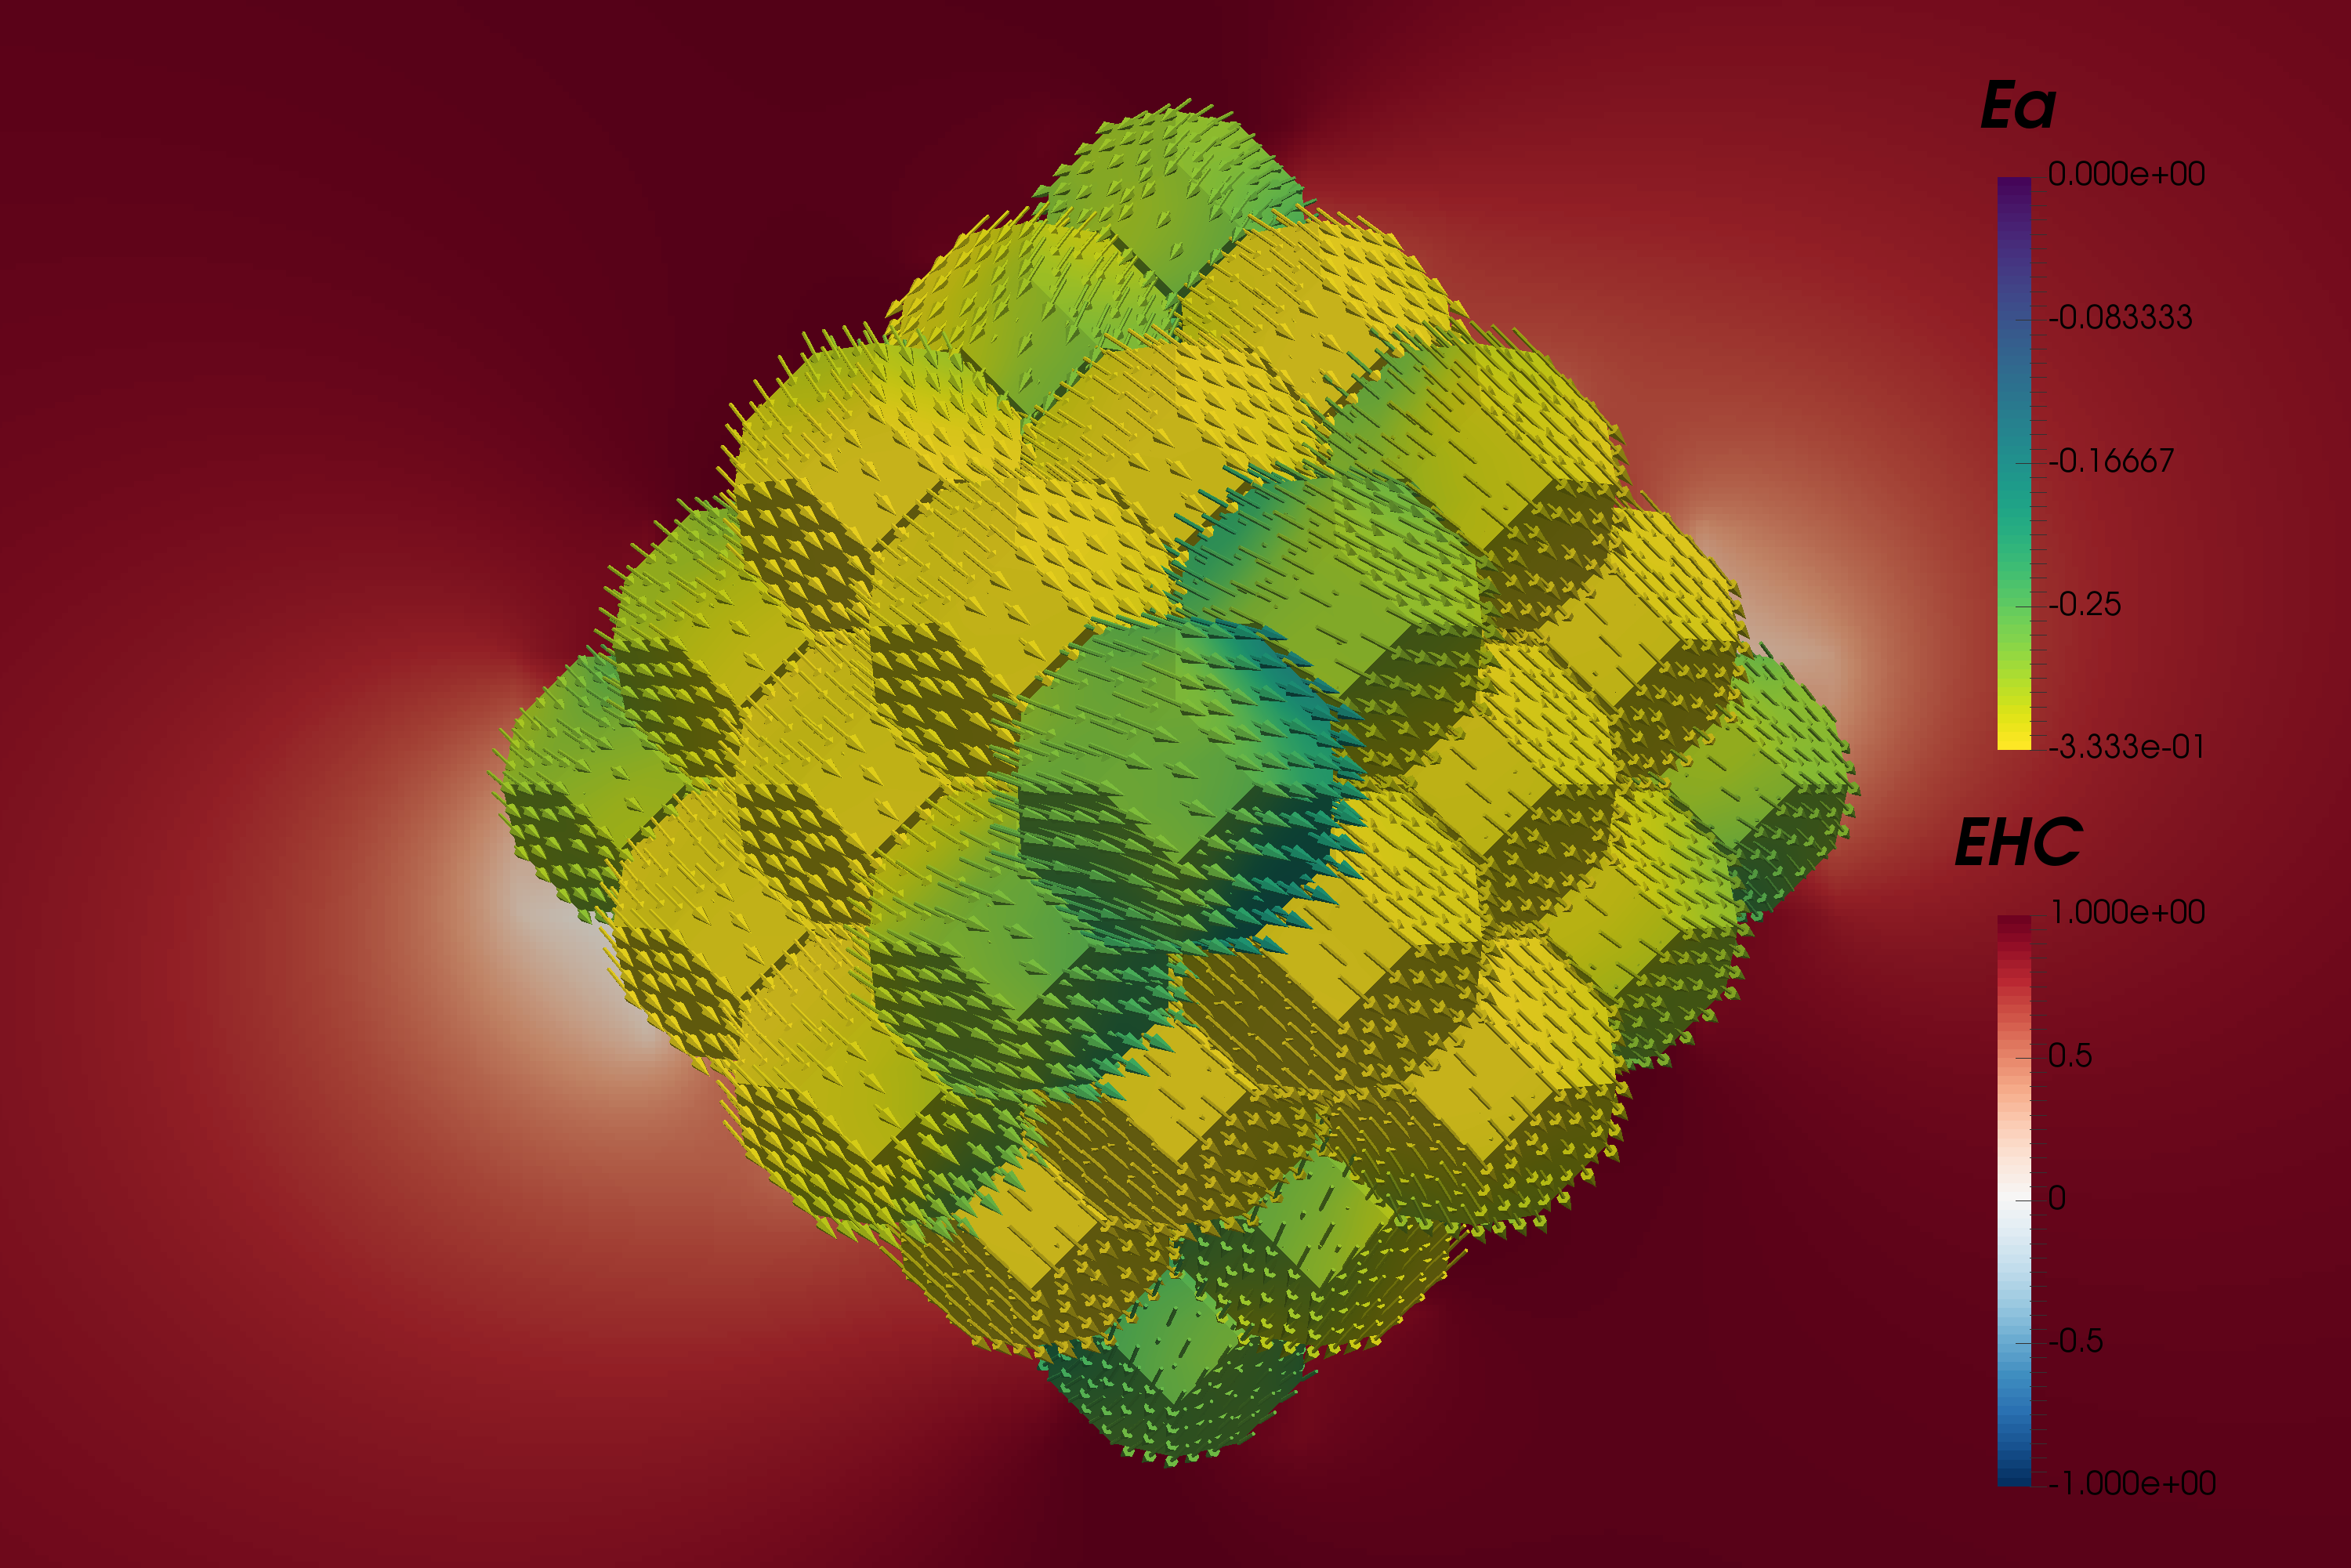
\includegraphics[width=\textwidth]{research-4/figs/fram_i16_f0_-y.png}
\caption[Remanent state when the field is along a hard axis (view from +Y)]{Remanent state when the field is along a hard axis (view from +Y).}
\label{FIG_23}
\end{figure}

\begin{figure}
\centering
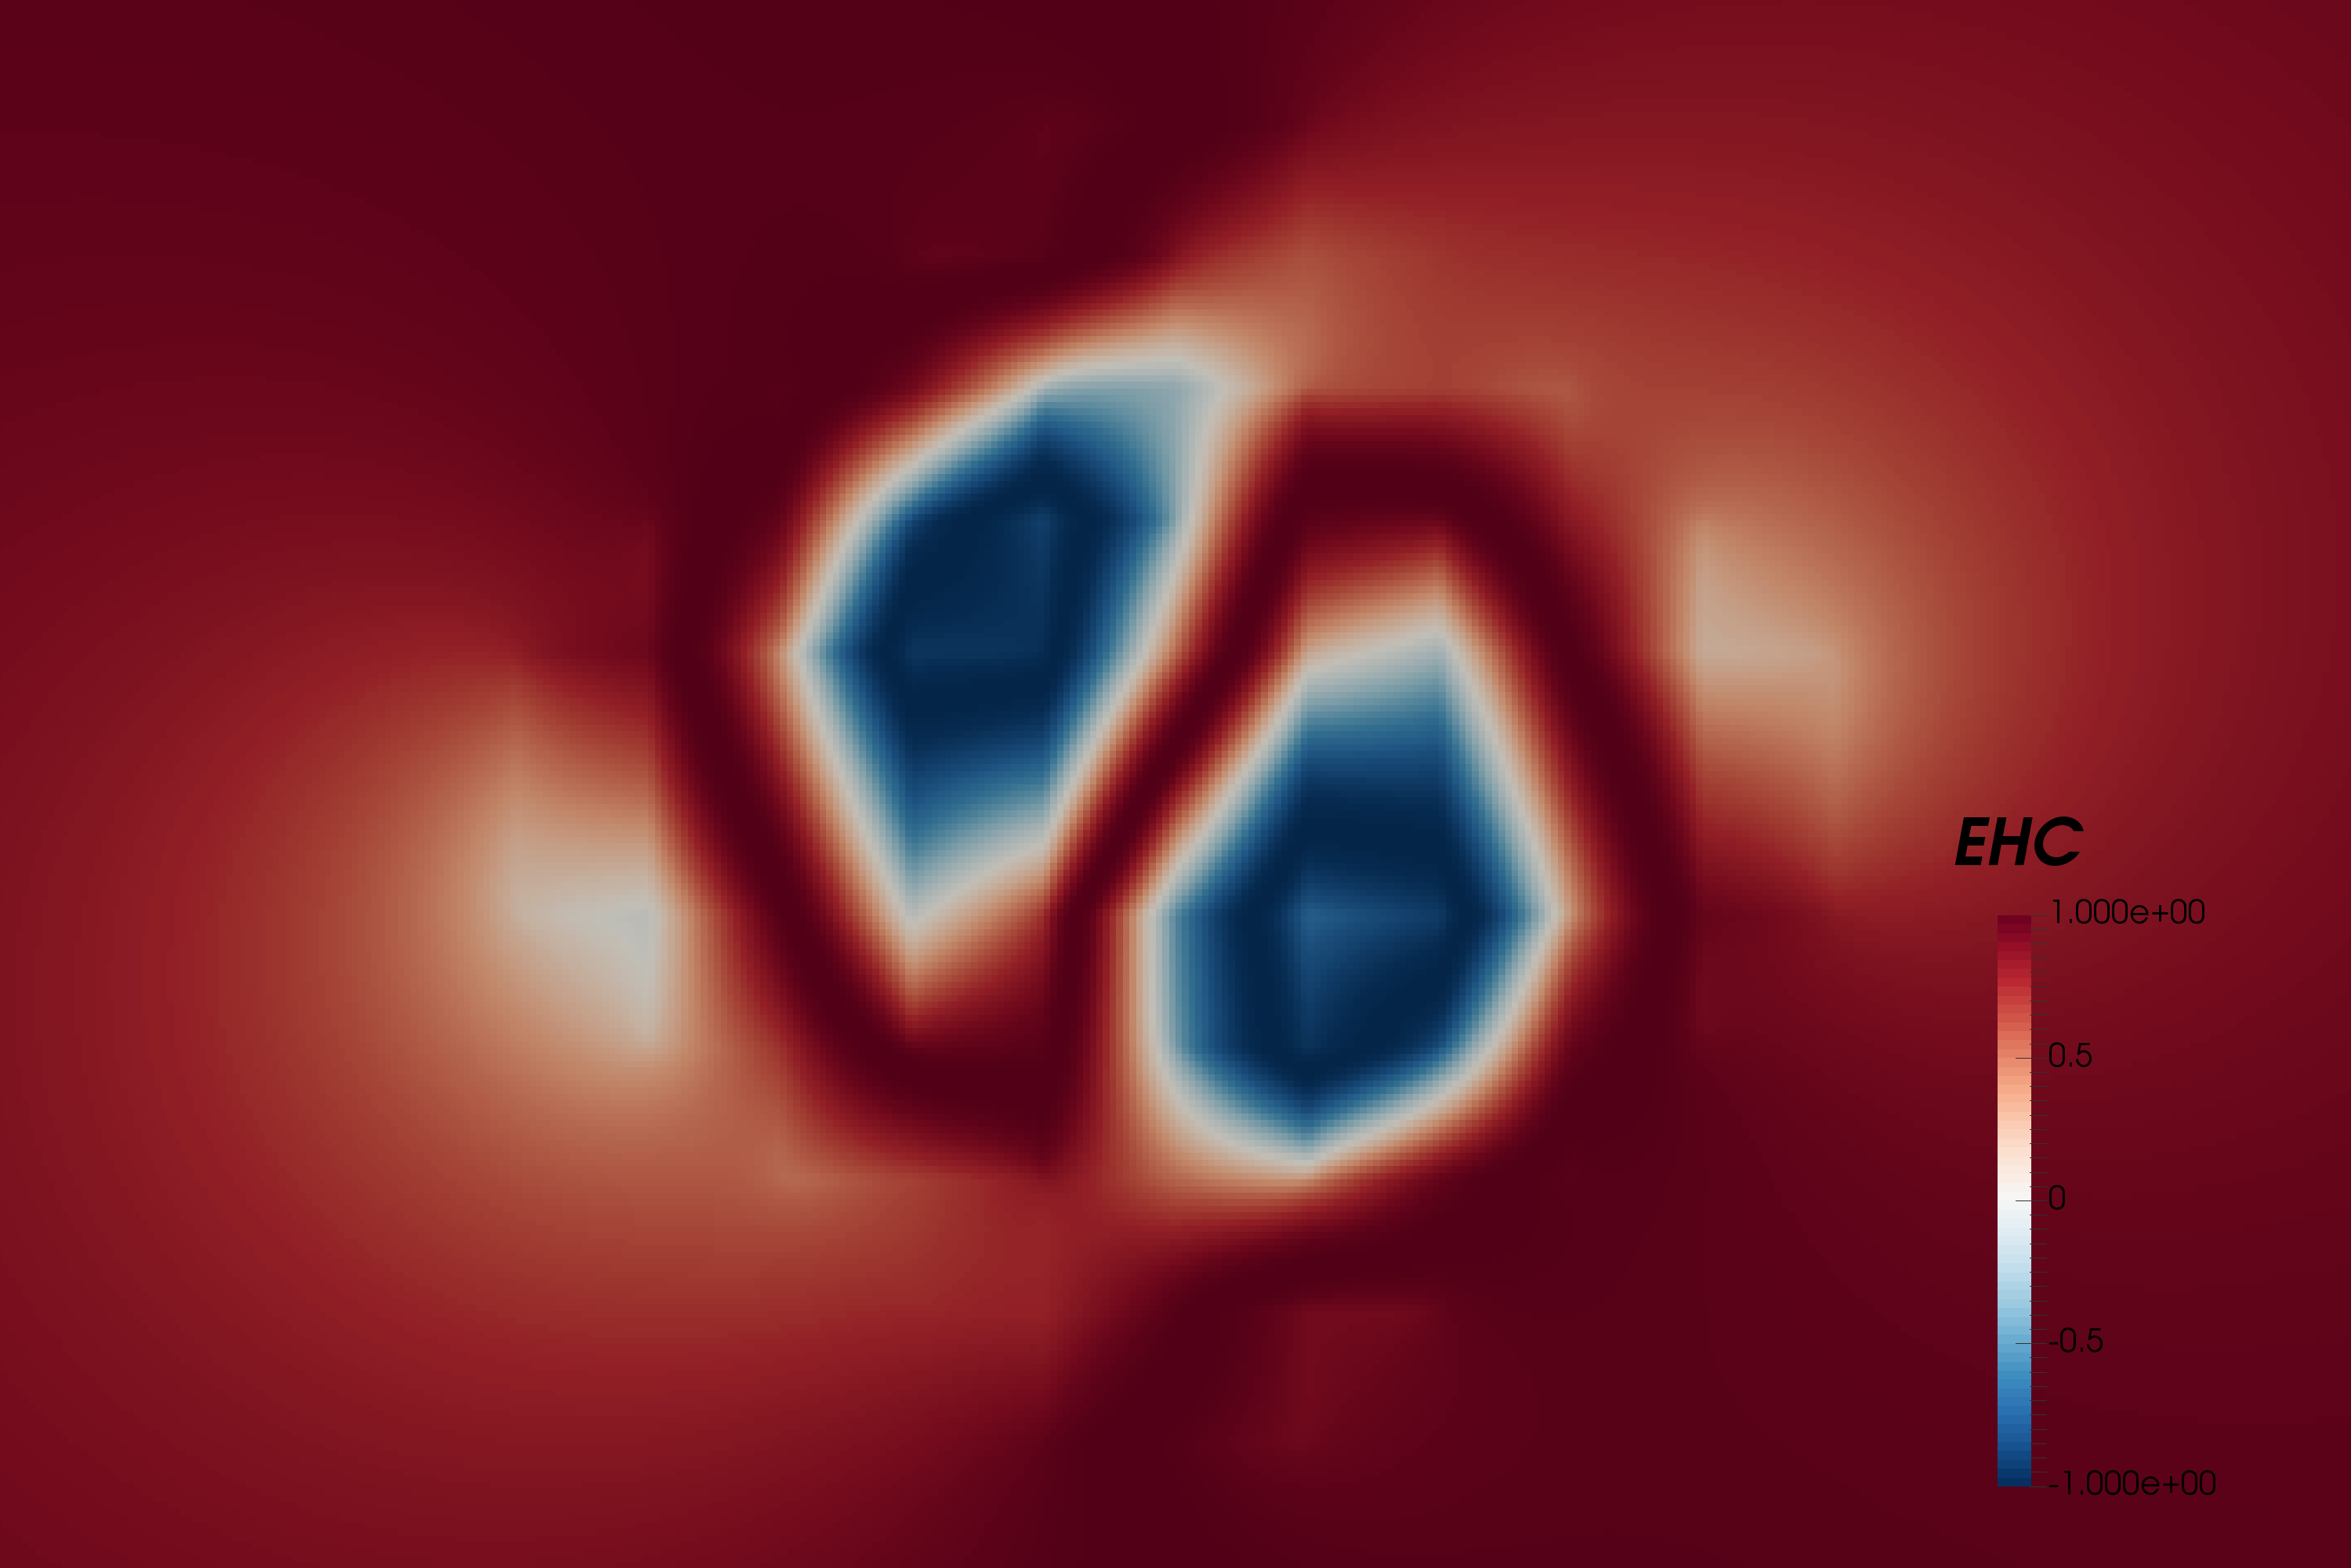
\includegraphics[width=\textwidth]{research-4/figs/fram_i16_f0_-y_EHC.png}
\caption[Electron holography map of the remanent state when the field is along a hard axis (view from +Y)]{Electron holography map of the remanent state when the field is along a hard axis (view from +Y).}
\label{FIG_24}
\end{figure}

\begin{figure}
\centering
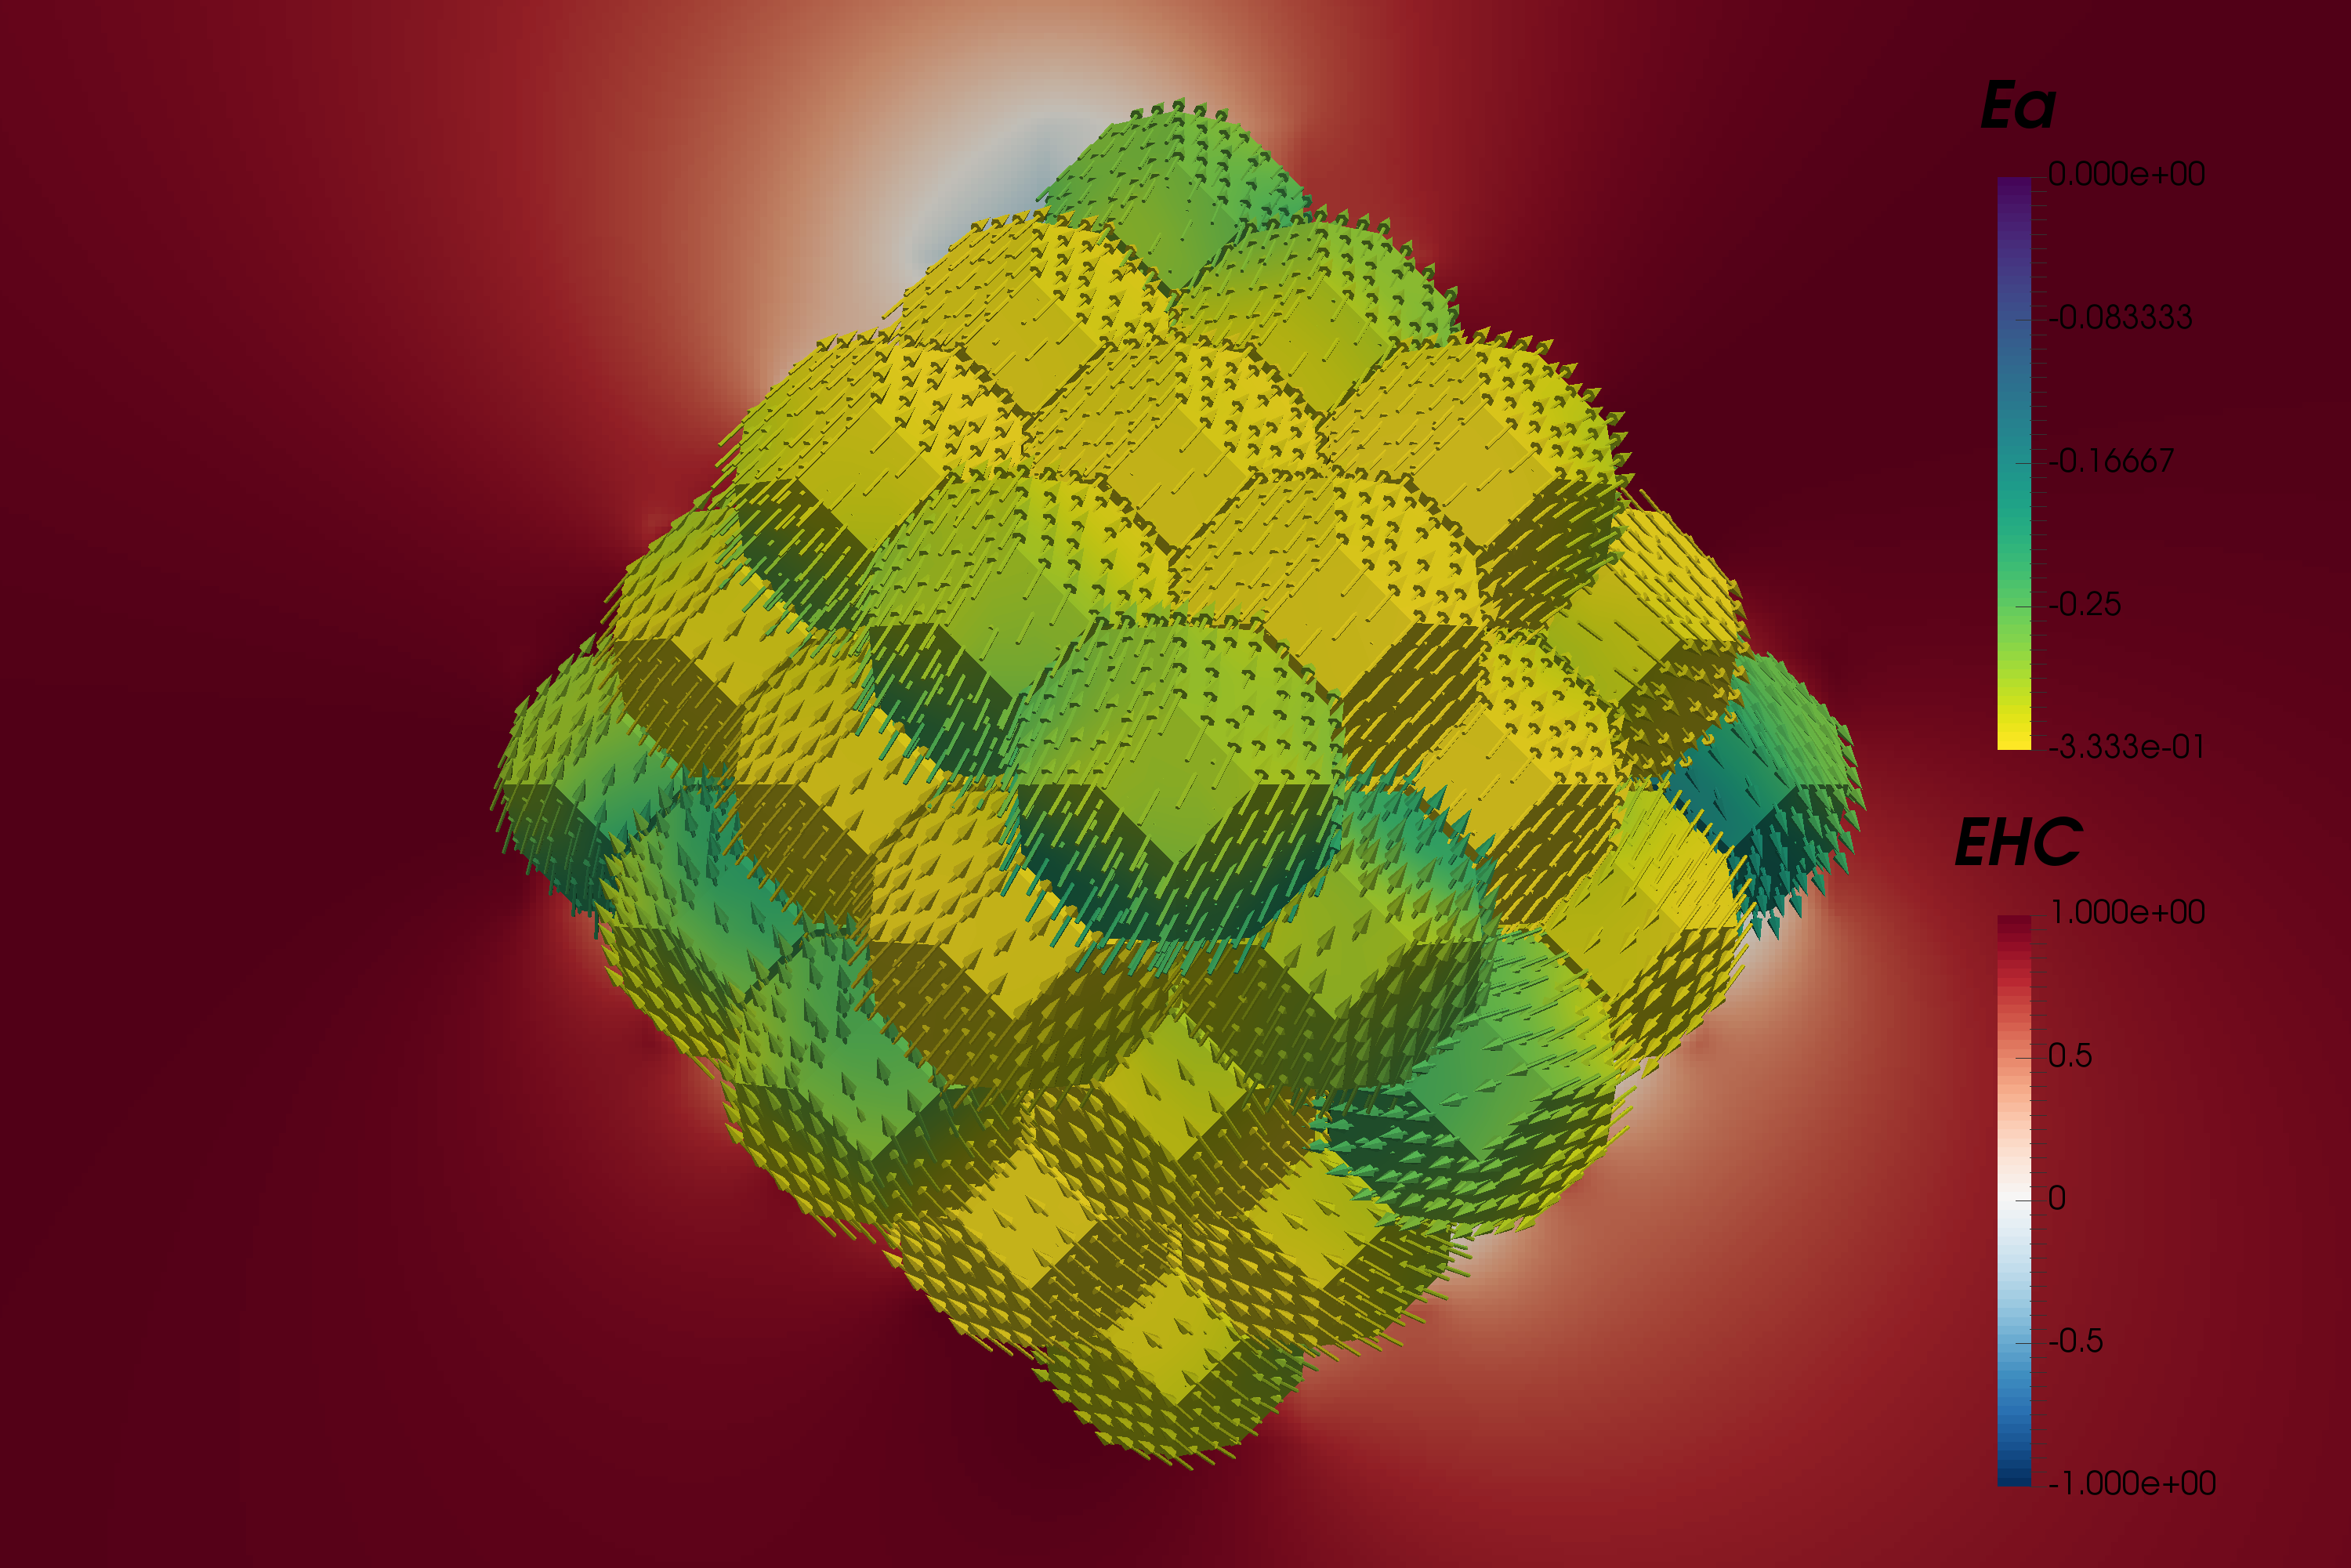
\includegraphics[width=\textwidth]{research-4/figs/fram_i16_f0_-x.png}
\caption[Remanent state when the field is along a hard axis (view from +X)]{Remanent state when the field is along a hard axis (view from +X).}
\label{FIG_25}
\end{figure}

\begin{figure}
\centering
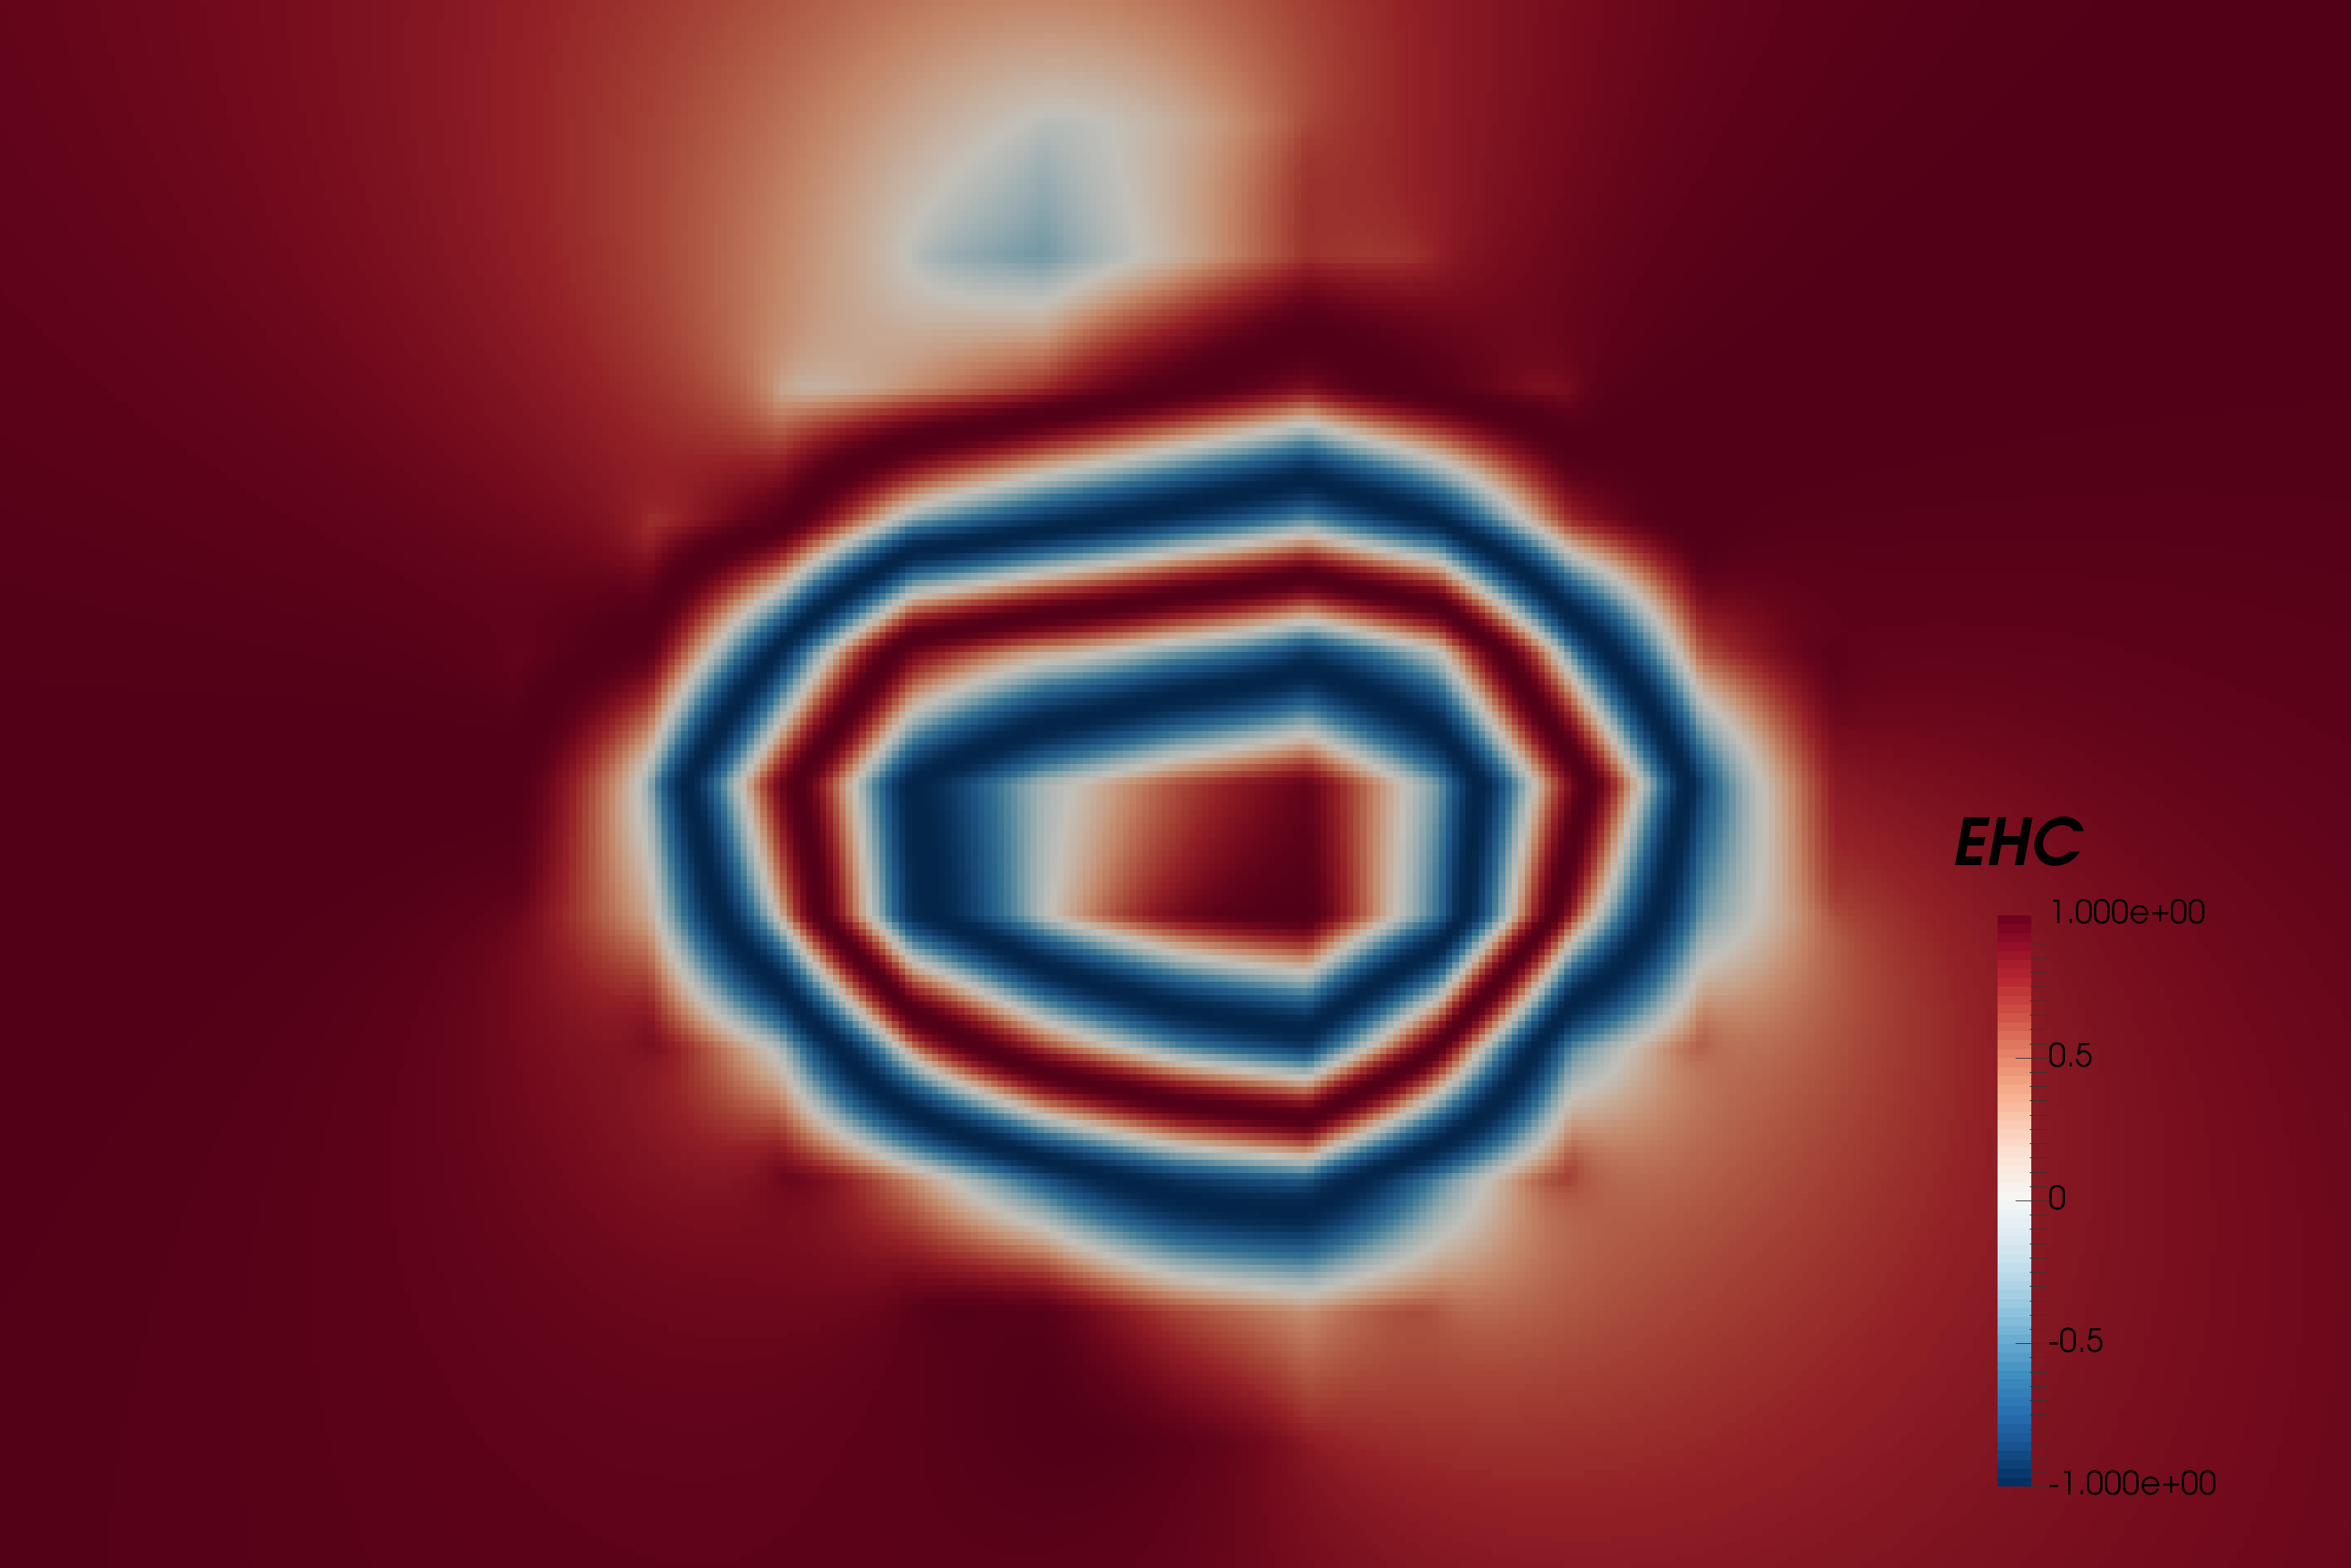
\includegraphics[width=\textwidth]{research-4/figs/fram_i16_f0_-x_EHC.png}
\caption[Electron holography map of the remanent state when the field is along a hard axis (view from +X)]{Electron holography map of the remanent state when the field is along a hard axis (view from +X).}
\label{FIG_26}
\end{figure}

\subsection{Hysteresis and remanent states of larger particle framboids.}
I calculated the hysteresis curves of smaller (less particles) framboids with 76$\nm$ particles (which are strictly SV when isolated) for the field directions I showed individual FORC diagrams for earlier in this chapter. I want to show here some of them and the remanent states with electron holography images. I had no time to finish those plots. The particles are not SD anymore, although the innermost particle does seem to remain SD during hysteresis.\par

\section{Discussion}
Discussion section...\par

\section{Conclusions}
Conclusion section...\par

%----------------------------------
\renewcommand\bibname{{References}}
\bibliographystyle{elsarticle-harv}
\bibliography{references}

